\documentclass[12pt,a4paper]{article}

\usepackage[T1,T2A]{fontenc}
\usepackage[utf8]{inputenc}
\usepackage[russian, english]{babel}
\usepackage{amsmath, amssymb, mathtools}
\usepackage[top=1in, bottom=1in, left=0.7in, right=0.7in]{geometry}
\usepackage{microtype}
\usepackage{indentfirst}
\usepackage{setspace}
\usepackage{enumitem}
\usepackage{booktabs}
\usepackage{float}
\usepackage{graphicx}
\usepackage{subcaption}
\usepackage{tabularx}
\usepackage[unicode=true, colorlinks=true, linkcolor=blue, urlcolor=blue, citecolor=blue]{hyperref}

\graphicspath{{../rl-credit-scoring-sim/outputs/}}
\setstretch{1.08}

\title{Контролируемое исследование размерности состояния\\для недельного управления кредитными порогами}
\author{}
\date{}

\begin{document}
\selectlanguage{russian}

\maketitle
\tableofcontents
\clearpage

\section{Введение}

Настоящий текст описывает актуальное состояние репозитория после того, как он был фактически перестроен вокруг контролируемого эксперимента по размерности состояния в задаче недельного управления порогами одобрения в кредитном скоринге. Это важно подчеркнуть сразу: исследование не сводится к обычной задаче бинарной классификации заявок и не сравнивает модели на статическом табличном датасете в стиле ``одобрить или отклонить отдельный объект''. В центре внимания находится динамическая портфельная политика. Контроллер раз в неделю выбирает пороги для новых и повторных клиентов, а затем именно эти недельные пороги определяют состав принятой когорты, будущие дефолты, возвраты, поздние recovery-потоки и, в конечном счете, финансовое качество всего портфеля.

Такая постановка делает исследование содержательно более близким к реальной практике управления кредитным потоком. В операционном процессе компания редко вручную пересматривает решение по каждой отдельной заявке как независимой единице. Намного типичнее ситуация, когда на определенный период времени задается или корректируется скоринговый cutoff, после чего бизнес наблюдает, как изменение этого cutoff влияет на объем выдач, качество новых когорт, нагрузку на капитал и последующие денежные потоки. Именно поэтому в репозитории объектом управления является не точечное решение по заемщику, а недельная пороговая политика.

Вторая принципиальная особенность исследования состоит в том, что финансовый результат здесь является \emph{отложенным}. Если кредит был выдан сегодня, его качество не раскрывается немедленно. Часть кредитов погашается позже, часть дефолтит, а часть дефолтов частично восстанавливается еще через несколько недель. Следовательно, нельзя оценивать политику по мгновенной выгоде текущей недели. Политика может выглядеть привлекательной локально, но оказаться слабой на полной траектории портфеля. И наоборот, более строгий режим одобрения может временно выглядеть хуже, зато на горизонте всей симуляции дать более чистый и устойчивый результат.

Текущий эксперимент в репозитории задает очень конкретный исследовательский вопрос: \emph{как меняется качество RL-контроллера, если увеличивать размер наблюдения с 12 до 20, 30 и 50 признаков, не меняя при этом остальные элементы постановки?} Такой вопрос ценен именно своей контролируемостью. Если меняется только \texttt{state\_dim}, то различия в результатах можно интерпретировать как различия в информативности и сложности пространства состояний, а не как следствие смены среды, набора сценариев, функции награды или конкурентных baseline-политик.

Поэтому главный вывод исследования должен формулироваться аккуратно. Репозиторий не показывает, что reinforcement learning уже однозначно превосходит все rule-based подходы. Наоборот, лучший overall-контроллер в quick-профиле остается не-RL baseline. Но репозиторий очень убедительно показывает другое: дизайн состояния существенно влияет на качество RL, рост размерности полезен лишь до определенного уровня, а польза от richer state сильно зависит от конкретного алгоритма.

\section{Что именно изучается и почему это важно}

\subsection{Почему исследуется именно недельное управление порогами}

Если смотреть на кредитный скоринг только как на задачу предсказания дефолта, то возникает соблазн считать, что все сводится к хорошей модели PD и выбору одного фиксированного threshold. Но в реальной кредитной политике этого недостаточно. Бизнес интересует не только точность ранжирования клиентов, но и то, как выбранная политика меняет будущую структуру портфеля. Важно не просто ``кого одобрить сегодня'', а ``какую недельную границу риска выдержит портфель так, чтобы одновременно не разрушить прибыльность, не разогнать дефолт и не перегрузить капитал''.

Именно поэтому в проекте действие контроллера определено как недельная пара порогов для новых и повторных клиентов. После выбора этих порогов симулятор генерирует поток заявок, применяет пороги, формирует принятую когорту, а далее разворачивает ее кредитную судьбу во времени. Такое представление делает задачу последовательной, стратегической и существенно более интересной, чем статическая классификация.

С исследовательской точки зрения это означает следующее. Во-первых, задача действительно становится reinforcement learning problem, потому что текущее решение влияет на будущее состояние портфеля. Во-вторых, качество политики можно обсуждать на языке, который близок к предметной области: прибыль, дефолтность, approval rate, capital usage, устойчивость награды, реакция на shift-сценарии.

\subsection{Почему отложенные исходы здесь принципиальны}

В обычной статической формулировке кредитный риск часто мыслится как функция от признаков клиента в момент принятия решения. В данной работе этого недостаточно, потому что исследование моделирует весь путь кредита после одобрения. Выданный займ не приносит окончательный финансовый результат сразу. Он живет несколько недель или месяцев, может привести к положительному cash flow, отрицательному default-loss, а затем, возможно, к позднему recovery.

Именно эта отложенность и делает задачу содержательной. Если бы награда зависела только от ожидаемой выгоды текущей когорты, контроллер можно было бы оценивать почти миопически. Но в текущей реализации награда с delayed reward опирается на \emph{реализованные} потоки, а не только на текущие ожидания. Это приводит к естественной исследовательской дилемме: политика, которая выглядит сильной ``здесь и сейчас'', может создать плохой хвост убытков позже; политика, которая в первые недели отстает, может оказаться лучше на полном горизонте.

В репозитории этот смысл подтверждается не только кодом, но и экспортированным диагностическим артефактом \texttt{outputs/dim\_30/locally\_worse\_globally\_better.csv}. Он показывает, что в adverse-stress среде некоторые агенты сначала проигрывают локально, а затем сильно выигрывают на финальной траектории. Например, для 30D DQN ранний разрыв зафиксирован примерно как $-643.46$, а финальный разрыв как $250{,}578.20$. Это не означает, что RL обязательно сильнее в stress-сценариях. Это означает другое: ранняя и итоговая оценка политики могут принципиально расходиться, а значит delayed-outcome логика является не декоративной, а методологически необходимой.

\subsection{Почему важно разделение на новых и повторных клиентов}

В среде новые и повторные заемщики не являются одним и тем же сегментом с переименованными колонками. Для них различаются параметры распределения скоринговых баллов, чувствительность default probability к score, вероятность recovery, размеры займа и сроки кредита. Это экономически реалистично: повторные клиенты обычно содержат дополнительный behavioral signal и нередко имеют другую риск-доходность, чем новые.

Из этого следует простой, но важный вывод: единый shared threshold может быть заведомо неэффективен. Поэтому split-policy логика здесь не второстепенная опция, а часть основной постановки. Контроллер в нормальном режиме выбирает не один порог, а пару порогов. Более того, один из сценариев специально построен так, чтобы новые клиенты ухудшались, а повторные, наоборот, улучшались. В такой среде полезность отдельного контроля по сегментам становится практически прямым предметом эксперимента.

Это особенно важно для темы размерности состояния. Рост числа признаков нужен не сам по себе. Он имеет смысл лишь тогда, когда добавляемые координаты помогают лучше описывать ту сложность, которая реально есть в задаче. В нашем случае такой сложностью являются сегментная неоднородность, история портфеля, лаги по прибыли и дефолту, gap между new и repeat thresholds, динамика капитальной нагрузки и т.д.

\section{Граница между reference-проектом и текущей реализацией}

Согласно \texttt{notes/reference\_study.md}, текущий проект сохраняет несколько ключевых идей исходной reference-работы: недельное взаимодействие, пороговое управление, delayed outcomes, delayed rewards, warm-up период и проверку устойчивости в shift-сценариях. Однако актуальный репозиторий нельзя описывать как простое воспроизведение старой схемы.

В текущей реализации появились важные расширения.
\begin{itemize}[leftmargin=*]
    \item Split-policy контроль для новых и повторных клиентов стал дефолтной логикой, а не частным случаем.
    \item Эксперименты стали config-driven: параметры профиля, горизонта, bootstrap CI и набора контроллеров задаются через текущие YAML-конфиги.
    \item Введен контролируемый эксперимент по размерности состояния, в котором сравниваются 12D, 20D, 30D и 50D наблюдения.
    \item Функция награды стала явно constraint-aware: она учитывает default-rate, approval-rate, capital-usage и volatility penalties.
    \item Набор RL-алгоритмов включает DQN, Double-DQN, PPO и SAC, а набор baseline-методов покрывает статические, миопические, реактивные и constraint-aware стратегии.
    \item В репозитории появились writer-handoff материалы, figure map, table map, экспорт CI-кривых и сводные кросс-размерные таблицы.
\end{itemize}

Для текста диплома это означает, что нельзя опираться на старую интуицию о ``простом одномерном state'' или ``едином пороге''. Источник истины теперь находится в текущем коде, конфигурации и экспортированных результатах.

\section{Как устроен симулятор}

\subsection{Временная структура эпизода}

В \texttt{src/rl\_credit\_scoring\_sim/env/simulator.py} эпизод разбит на три логические фазы.
\begin{enumerate}[leftmargin=*]
    \item \textbf{Warm-up.} В течение 8 недель симулятор работает на дефолтных порогах, чтобы сформировать начальный пул незавершенных кредитов, rolling-метрики прибыли и исторические показатели дефолтов.
    \item \textbf{Interactive horizon.} Затем начинаются 26 интерактивных недель quick-профиля, в которых контроллер реально управляет порогами.
    \item \textbf{Terminal settlement.} После завершения интерактивного горизонта все оставшиеся interactive-cashflow события закрываются, чтобы эпизод не обрывался искусственно на середине жизненного цикла недавно выданных кредитов.
\end{enumerate}

Последний пункт особенно важен. Без terminal settlement политика, которая в конце эпизода активно выдает длинные кредиты, систематически выглядела бы хуже, чем есть на самом деле, потому что положительные потоки по этим кредитам просто не успели бы попасть в measured horizon. Текущая реализация корректирует эту проблему.

\begin{figure}[H]
    \centering
    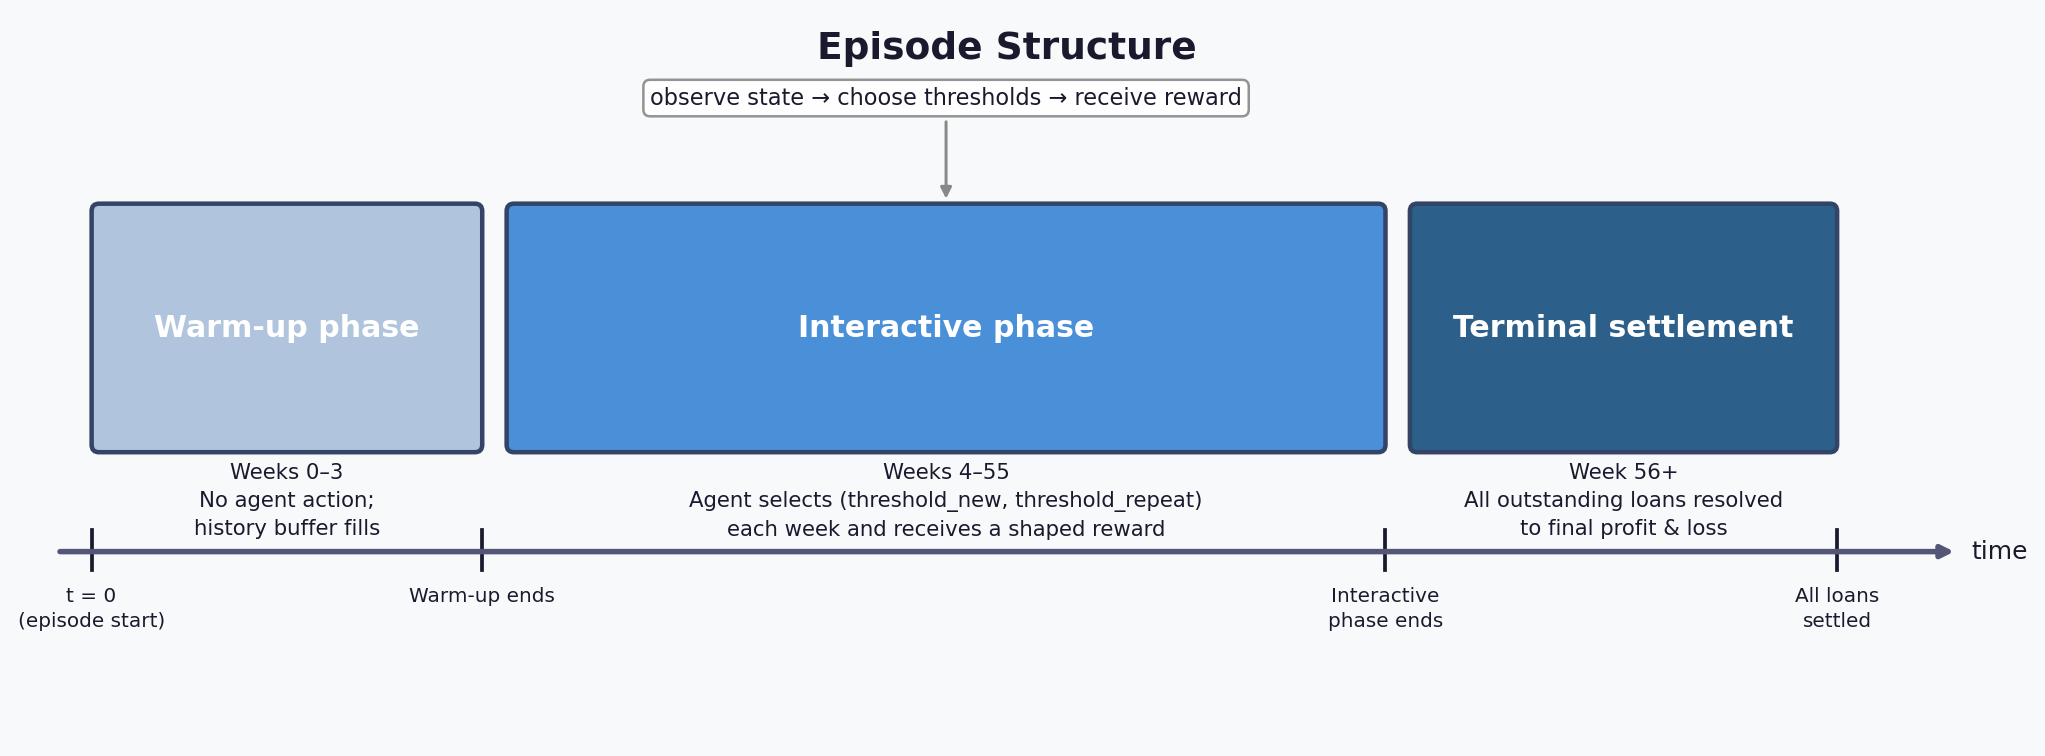
\includegraphics[width=0.92\textwidth]{diagrams/episode_timeline.png}
    \caption{Трёхфазная структура эпизода. Фаза warm-up заполняет кредитную книгу до начала управления; интерактивная фаза --- горизонт принятия решений агентом; terminal settlement закрывает все незавершённые кредиты, чтобы итоговые метрики отражали реальные последствия политики.}
    \label{fig:ru-episode-timeline}
\end{figure}

\subsection{Что происходит внутри одной недели}

Каждая неделя начинается с формирования scenario-specific market state. Сценарий задает динамику доли repeat-клиентов, тренд объемов, сезонность, сдвиги score distributions, сдвиги default pressure, уровень шума, коэффициент размера займа, качество recovery и параметры shock-эпизода.

После этого симулятор генерирует weekly application counts отдельно для новых и повторных клиентов, рисует score distributions, строит default probabilities через сегментные sigmoid-функции, определяет will-default / will-recover траектории и задает loan amount и duration. Далее выбранные пороги применяются к обоим сегментам. Все заявки с score выше соответствующего порога принимаются.

Именно на этом месте проявляется главная экономическая идея исследования. Одобренные кредиты не сразу превращаются в итоговую прибыль. Они лишь создают будущие события: repayment, default-loss и, при необходимости, late recovery. Поэтому в текущей неделе одновременно существуют два разных типа информации.
\begin{itemize}[leftmargin=*]
    \item Характеристики \emph{текущей принятой когорты}: \texttt{expected\_profit\_current}, \texttt{expected\_npv\_current}, \texttt{expected\_default\_rate\_current}.
    \item \emph{Реализованные} потоки по ранее выданным кредитам: \texttt{realized\_profit}, \texttt{realized\_npv}, realized default counts и т.д.
\end{itemize}

Такое разделение делает симулятор методологически сильнее. Он не смешивает сегодняшние ожидания и сегодняшние реализованные потоки, а позволяет анализировать, как текущее решение будет раскрывать себя во времени.

\begin{figure}[H]
    \centering
    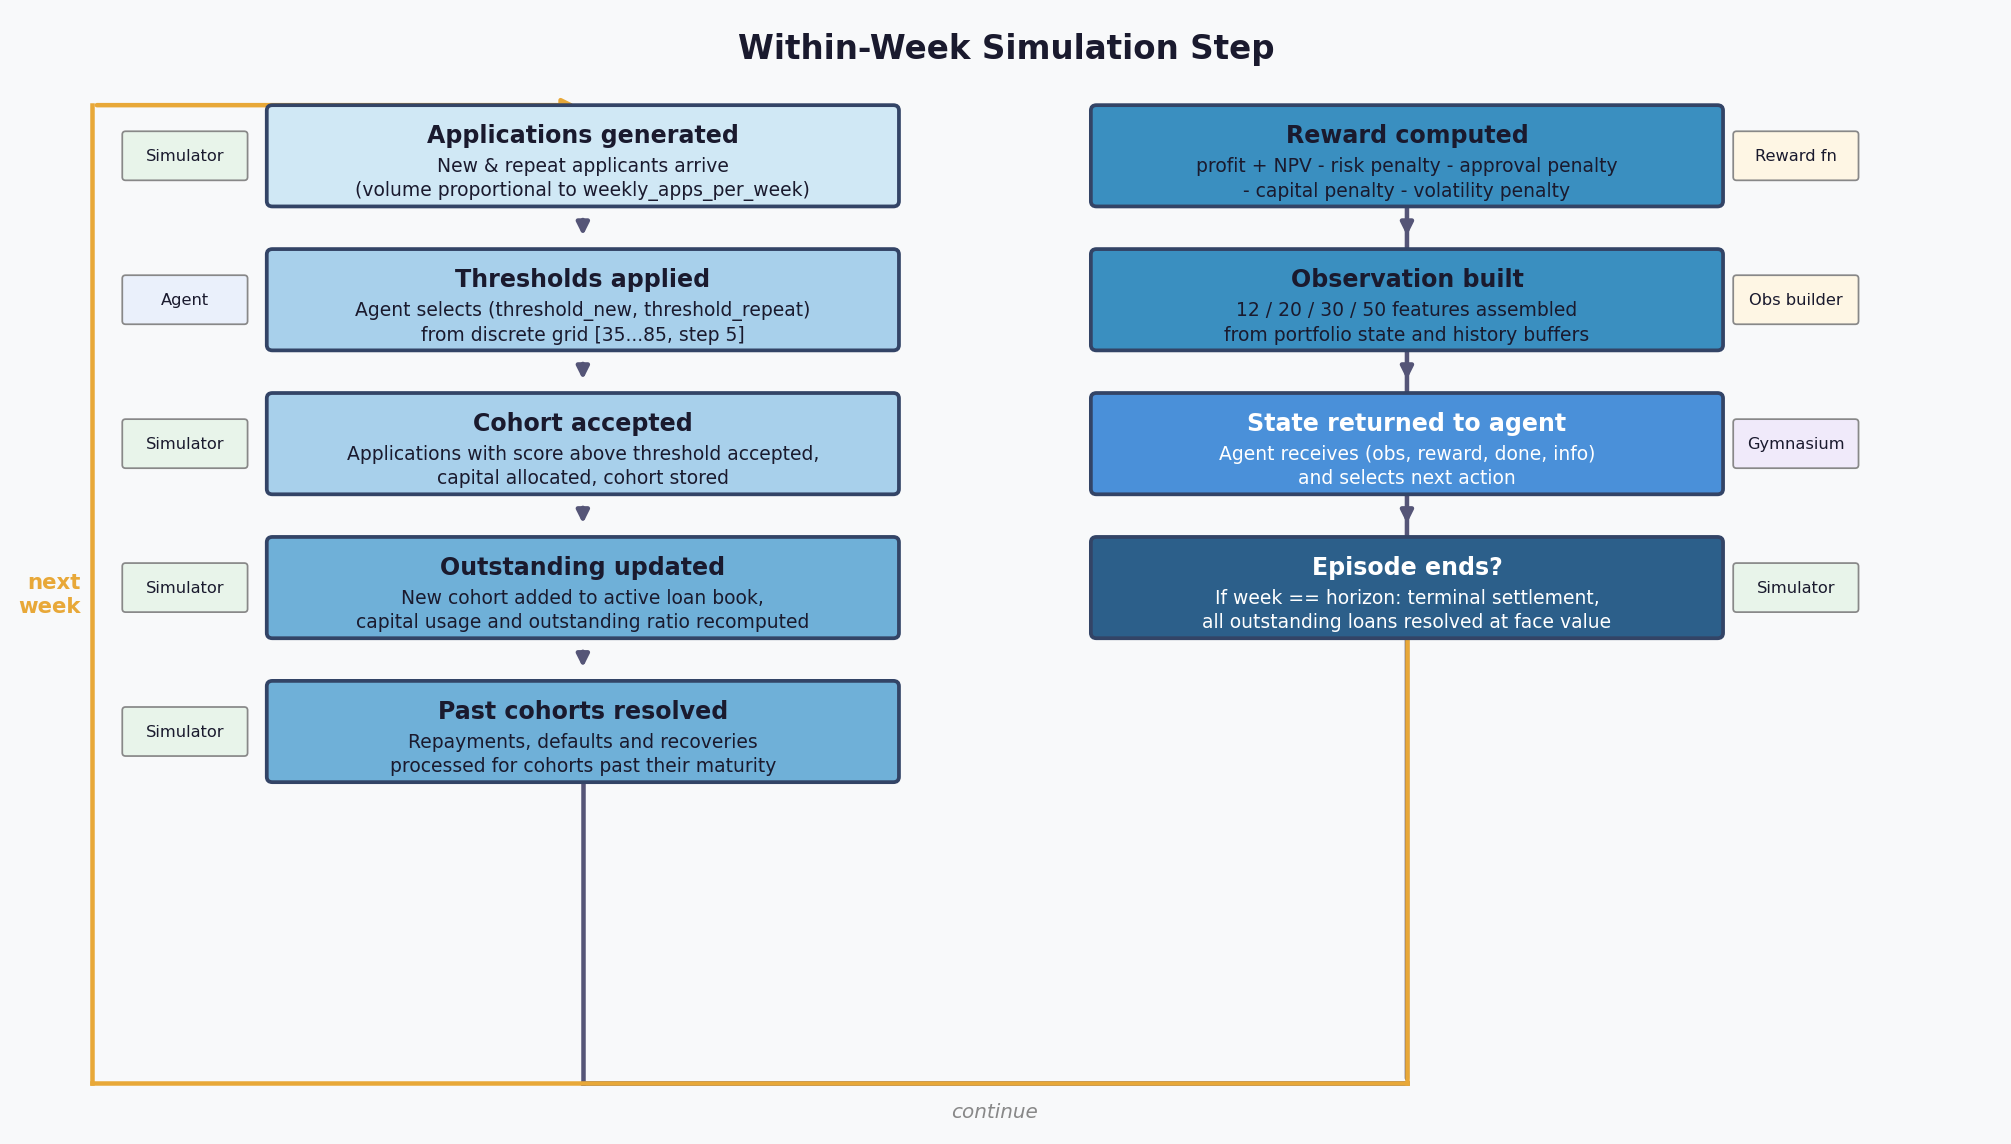
\includegraphics[width=0.96\textwidth]{diagrams/weekly_flowchart.png}
    \caption{Последовательность шагов внутри одной недели. Девять этапов разбиты на два столбца: шаги~1--5 слева (генерация рынка и управление когортами) и шаги~6--9 справа (вычисление награды, построение наблюдения, проверка терминального условия). Нижний мост соединяет шаг~5 с шагом~6; оранжевый путь слева показывает переход от шага~9 обратно к шагу~1 в начале следующей недели.}
    \label{fig:ru-weekly-flowchart}
\end{figure}

\subsection{Моделирование данных и симуляция}

Поскольку реальные данные на уровне кредитов с отложенными исходами
погашения недоступны в требуемой детализации, в работе используется
синтетический симулятор, откалиброванный по опубликованной статистике
розничного кредитования. Каждую неделю симулятор генерирует пул заявок
из параметрических распределений скоров отдельно для новых и повторных
клиентов. Заявки выше порога принятия одобряются; отклонённые заявки
отбрасываются без дальнейшего отслеживания.

Одобренные кредиты попадают в конвейер отложенного погашения: кредит,
выданный на неделе~$t$, может получить дефолт на неделе~$t + \Delta$,
где~$\Delta$ подчиняется фиксированному распределению лагов, отражающему
типичные паттерны seasoning розничных кредитов. Эта задержка является
центральным элементом исследовательского вопроса: агент наблюдает
последствия своих пороговых решений лишь спустя несколько недель,
а не немедленно.

\begin{figure}[H]
    \centering
    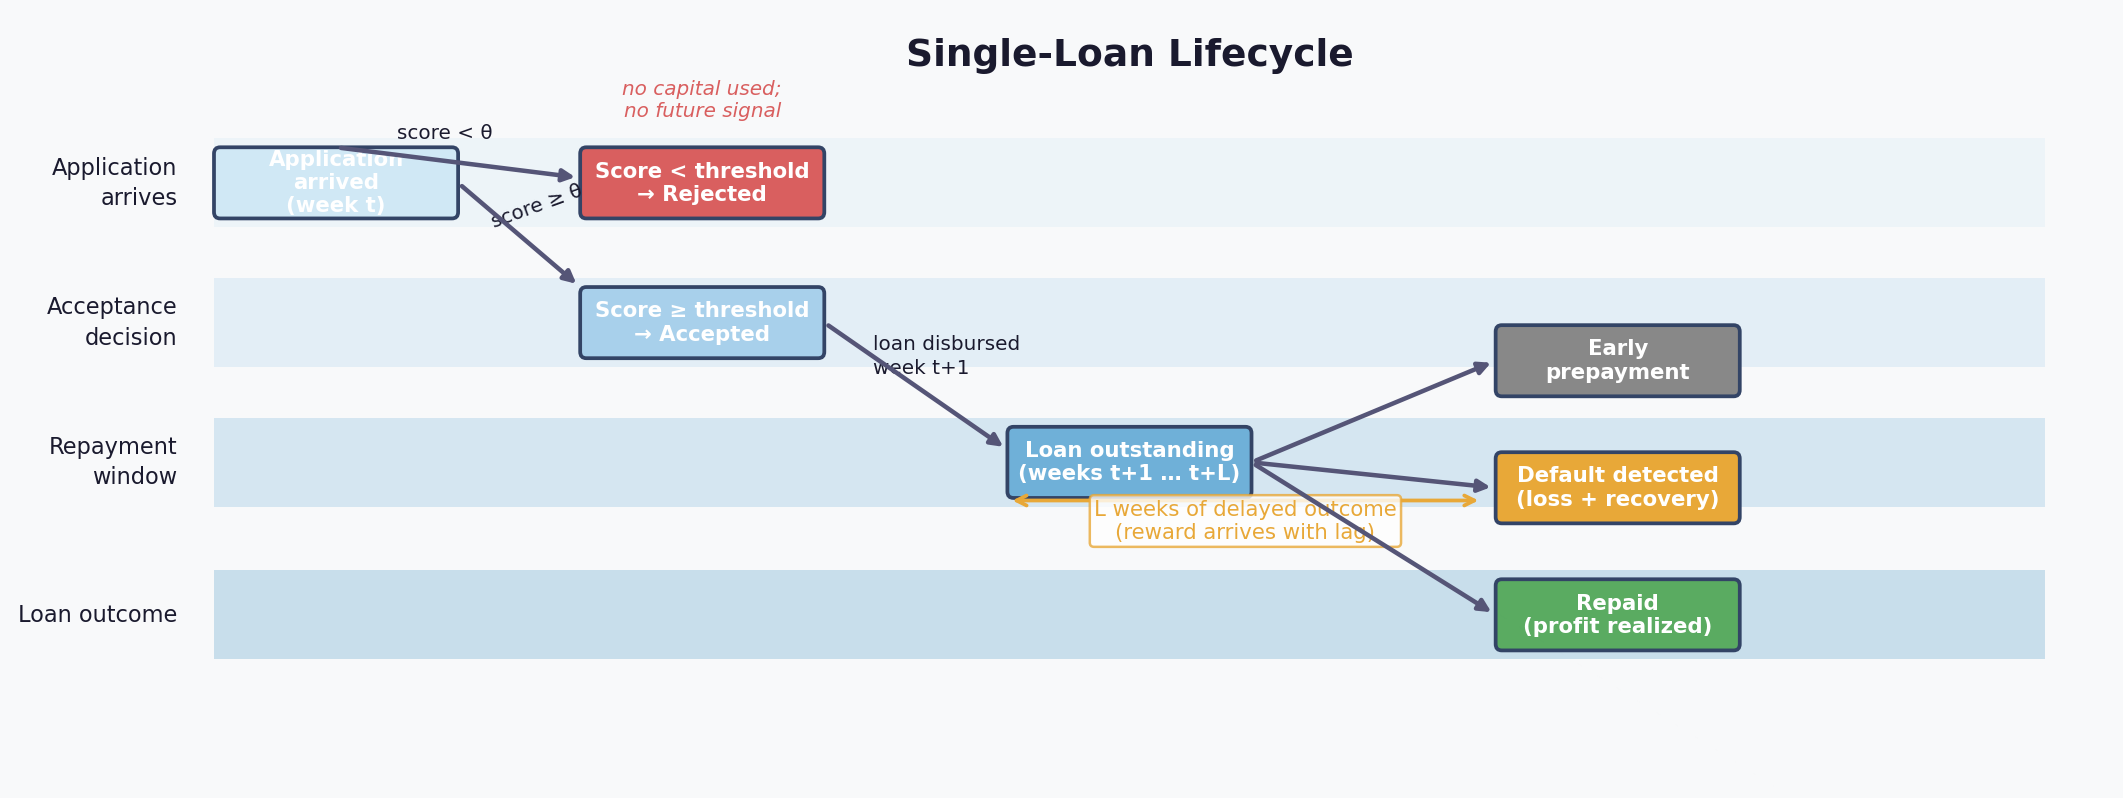
\includegraphics[width=0.92\textwidth]{diagrams/loan_lifecycle.png}
    \caption{Жизненный цикл отдельного кредита. Заявка, поступившая на неделе~$t$, либо отклоняется (скор ниже порога, дальнейшего учёта нет), либо принимается. Принятые кредиты остаются в книге в течение $L$~недель и завершаются погашением, дефолтом или досрочным возвратом. Именно окно задержки~$L$ порождает проблему кредитного присвоения во времени.}
    \label{fig:ru-loan-lifecycle}
\end{figure}

Вероятности дефолта откалиброваны по опубликованным данным розничного
кредитования. В базовом сценарии целевой уровень дефолтности портфеля
составляет 4--6\%, что соответствует работающим розничным кредитным
портфелям согласно данным ЦБ РФ (форма~0409115) и отчётам по кредитным
потерям ЕЦБ (ECB SSM). Стрессовые сценарии достигают 9--14\%, что
согласуется с кризисными наблюдениями в потребительском кредитовании.

\begin{figure}[H]
    \centering
    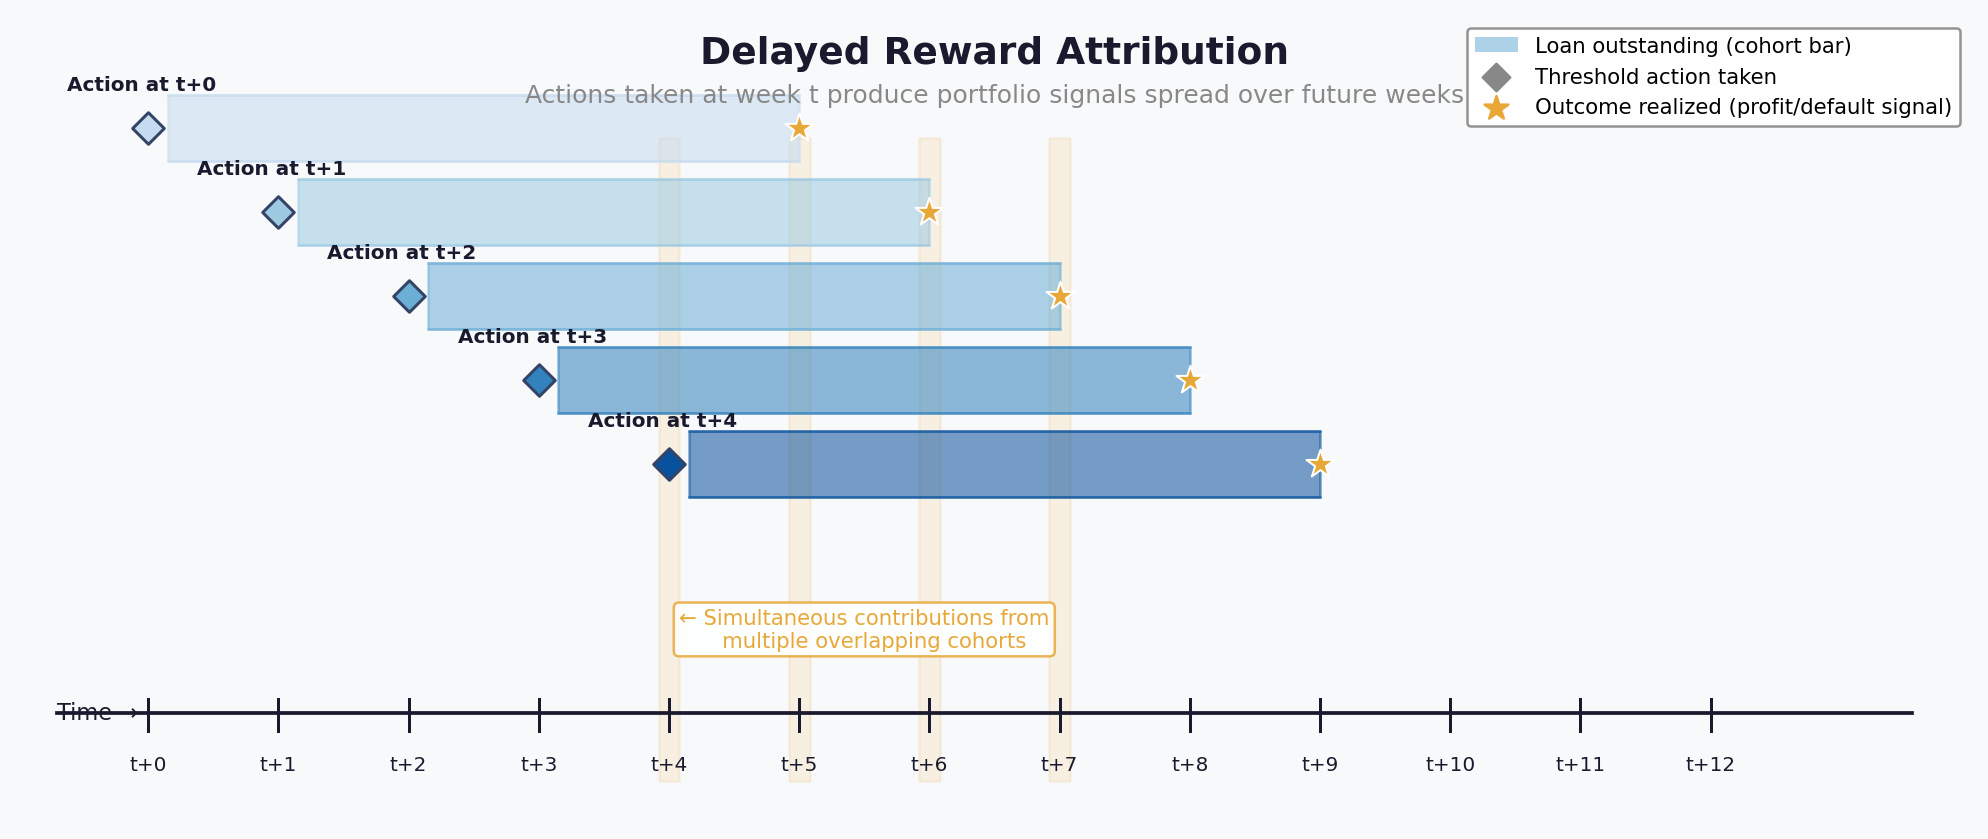
\includegraphics[width=0.92\textwidth]{diagrams/delayed_reward.png}
    \caption{Атрибуция отложенной награды. Каждая полоса соответствует когорте кредитов, принятых на определённой неделе (маркер-ромб); когорта остаётся активной в течение $L$~недель, после чего фиксируется исход (маркер-звезда). На любой данной неделе сигналы прибыли и дефолтов поступают одновременно от нескольких перекрывающихся когорт разных периодов выдачи, что усложняет задачу обучения агента.}
    \label{fig:ru-delayed-reward}
\end{figure}

\subsection{Уточнение по метрике \texttt{expected\_profit}}

Важная деталь, которую нужно зафиксировать в тексте диплома: экспортированные CSV-файлы сохраняют название \texttt{expected\_profit\_mean}, но в текущем коде агрегированная episode-level метрика вычисляется как сумма \emph{реализованной} прибыли по интерактивным неделям плюс terminal settlement. Иными словами, это legacy-name, а не буквальное ``математическое ожидание прибыли'' в узком смысле.

Поэтому в интерпретации результатов удобно делать так: при ссылке на конкретные CSV можно сохранять repository terminology и говорить \texttt{expected\_profit\_mean}, но содержательно пояснять, что это итоговая реализованная прибыль портфеля внутри эпизода. Такое уточнение согласует текст с реальным кодом \texttt{episode\_summary()} и убирает возможную терминологическую путаницу.

\section{Сценарии и их исследовательский смысл}

Шесть активных сценариев описаны в \texttt{configs/scenarios.yaml}. Они нужны не просто для визуального разнообразия. Каждый сценарий проверяет определенный механизм управления.

\begin{table}[H]
    \centering
    \small
    \begin{tabularx}{0.98\textwidth}{p{0.20\textwidth}X}
        \toprule
        Сценарий & Что именно он проверяет \\
        \midrule
        \texttt{base\_market} & Стабильный рынок без сильной структурной поломки. Это лучший сценарий для проверки, умеет ли контроллер использовать информативное состояние без борьбы с резким regime shift. \\
        \texttt{drift} & Медленное ухудшение качества, прежде всего у новых клиентов, плюс рост объема. Проверяется способность уловить постепенную деградацию и стать более селективным до того, как портфель существенно испортится. \\
        \texttt{adverse\_stress} & Резкий негативный shock, более высокие дефолты, шум и повышенный pressure на капитал. Здесь наказываются слишком агрессивные политики. \\
        \texttt{class\_imbalance\_shift} & Ускоренный рост доли более слабого сегмента новых клиентов. Сценарий показывает, насколько политика умеет работать не только с общим approval rate, но и с composition risk. \\
        \texttt{noise} & Более высокий measurement noise и нестабильные weekly volumes. Это тест на устойчивость к шуму и случайным колебаниям входного потока. \\
        \texttt{split\_policy\_dynamics} & Новые клиенты ухудшаются, а повторные улучшаются. Это самый прямой тест полезности split thresholds и сегментно-специфического состояния. \\
        \bottomrule
    \end{tabularx}
    \caption{Логика сценариев из \texttt{configs/scenarios.yaml}.%
    \protect\footnote{Целевые показатели дефолтности откалиброваны по опубликованным
    данным розничного кредитования: базовый сценарий (4--6\%) соответствует
    показателям работающего портфеля согласно данным ЦБ РФ (форма 0409115);
    сценарий стресса (9--14\%) --- кризисным периодам по данным ЕЦБ и
    индексам потребительских ABS Moody's.}}
    \label{tab:ru-scenarios}
\end{table}

Именно наличие этих сценариев позволяет осмысленно обсуждать, \emph{почему} один и тот же контроллер выигрывает в одних режимах и проигрывает в других. Без сценарной структуры весь анализ свелся бы к безликой средней метрике, что сильно обеднило бы научную интерпретацию.

\section{Контролируемый эксперимент по размерности состояния}

\subsection{Что зафиксировано}

Сильная сторона текущего репозитория состоит в том, что эксперимент действительно сделан controlled. Во всех четырех запусках постоянными остаются:
\begin{itemize}[leftmargin=*]
    \item среда, сценарии и недельная логика симуляции;
    \item split-policy action semantics;
    \item диапазон порогов от 35 до 85 с шагом 5;
    \item delayed reward, risk-aware shaping и penalty logic;
    \item warm-up, interactive horizon и terminal settlement;
    \item seeds 11, 23, 37;
    \item train/eval protocol и набор контроллеров;
    \item bootstrap-CI логика и формат экспортируемых артефактов.
\end{itemize}

Это делает эксперимент содержательно чистым. Когда меняется только \texttt{state\_dim}, можно честно говорить об эффекте размерности состояния, а не о сумме несогласованных изменений.

\subsection{Что меняется}

Единственный экспериментальный фактор:
\[
    \texttt{state\_dim} \in \{12, 20, 30, 50\}.
\]

Причем рост размерности сделан кумулятивно: 20D содержит весь 12D baseline и добавляет новый слой, 30D содержит 20D и добавляет исторические признаки, 50D содержит 30D и добавляет более богатые сегментные и stability-признаки.

\subsection{Как устроены слои состояния}

Пространство наблюдений сконструировано в четырёх последовательных слоях
согласно принципу \textit{информационной достаточности без look-ahead bias}:
каждый слой добавляет только ту информацию, которую риск-менеджер
реалистично наблюдает в момент принятия недельного решения, без доступа
к будущим исходам.

Послойная структура служит методологической цели, выходящей за рамки
простого feature engineering: удерживая все остальные экспериментальные
факторы постоянными (динамику среды, функцию награды, архитектуры агентов,
протокол оценки и random seeds) и варьируя только размерность наблюдения,
мы получаем контролируемое измерение того, как информационное богатство
влияет на качество RL-политики в задаче кредитного управления с отложенными
исходами.

Четыре слоя таковы: (1)~12-мерная операционная панель, представляющая
минимально достаточное недельное состояние; (2)~20-мерное расширение,
добавляющее текущий экономический контекст и forward-looking сигналы;
(3)~30-мерное состояние с исторической памятью, включающее лаги и rolling
статистики для темпоральной адаптации; и (4)~50-мерное состояние с богатой
сегментацией, разделяющее сигналы новых и повторных клиентов детально.
Предполагается, что качество растёт от 12D к 30D (информационный прирост
превышает шум оценки), а затем выходит на плато от 30D к 50D вследствие
убывающей отдачи при ограниченном training budget --- гипотеза, формально
проверяемая как H1.

\begin{table}[H]
    \centering
    \small
    \begin{tabularx}{0.98\textwidth}{p{0.11\textwidth}X}
        \toprule
        Размер & Содержательная интерпретация \\
        \midrule
        12D & Компактная недельная панель: где находится эпизод, какой был approval rate, как выглядит rolling realized default, какова текущая profit/volatility картина, каков capital pressure и какие thresholds применялись. \\
        20D & 12D плюс немедленный экономический контекст: expected profit и expected NPV на заявку, realized NPV, weekly reward, repeat-share, threshold gap и headroom по капиталу. \\
        30D & 20D плюс память о недавней истории: лаги approval/default/profit/capital usage, rolling averages, rolling std по прибыли и lagged threshold deltas. \\
        50D & 30D плюс более детализированное сегментное и stability-описание: segment-specific approval/default/profit признаки, доли принятых новых и повторных клиентов, rolling reward moments, cumulative profit/reward to date, volatility капитальной нагрузки и история threshold-gap. \\
        \bottomrule
    \end{tabularx}
    \caption{Смысл слоев состояния. Точный порядок признаков и их определения даны в \texttt{state\_dimension\_manifest.md}.}
    \label{tab:ru-features}
\end{table}

\begin{figure}[H]
    \centering
    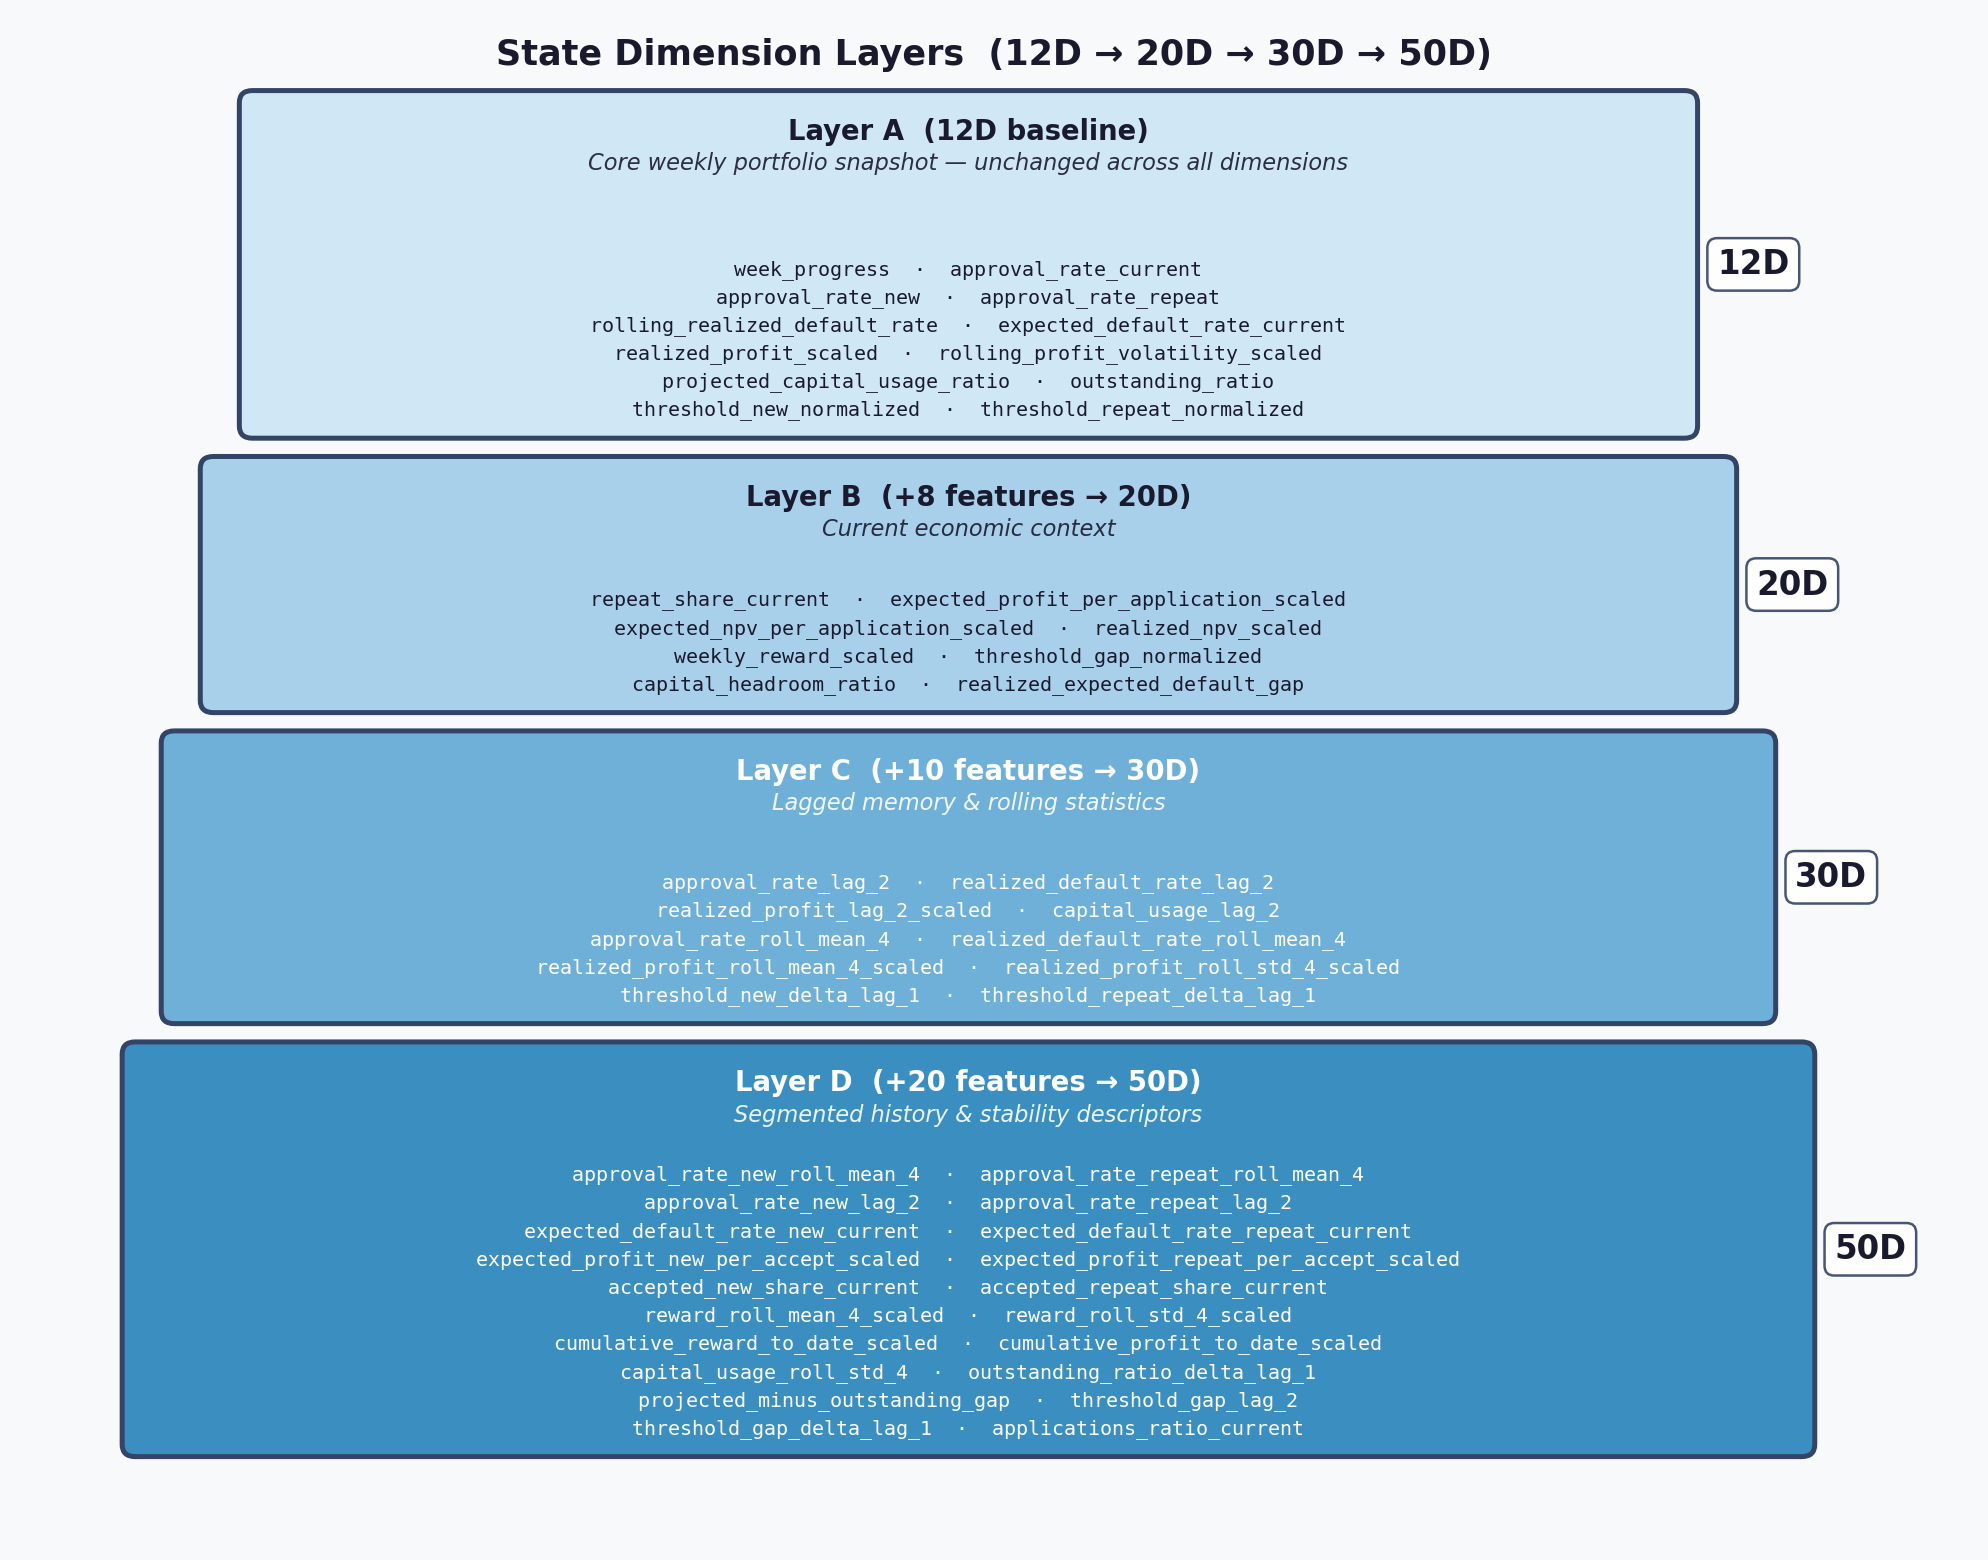
\includegraphics[width=0.92\textwidth]{diagrams/state_dimension_layers.png}
    \caption{Кумулятивные слои пространства состояния. Слой~A (12D) --- инвариантный базовый уровень, присутствующий во всех конфигурациях. Слои~B, C и~D последовательно добавляют экономический контекст, историческую память и сегментированные признаки. Первые 12~признаков тождественны во всех четырёх конфигурациях; это свойство проверяется программно перед каждым запуском эксперимента.}
    \label{fig:ru-state-layers}
\end{figure}

Очень важно, что в коде есть отдельная programmatic check, подтверждающая неизменность первых 12 признаков между 12D, 20D, 30D и 50D. Для научной добросовестности это принципиально: эксперимент не должен ``тихо'' менять baseline-ядро состояния, пока заявляет, что сравнивает только расширения.

\subsection{Почему дополнительные признаки вообще могут помочь}

Растущая размерность в этой работе не является бессодержательным увеличением числа координат. Добавляемые признаки имеют конкретный экономический смысл.
\begin{itemize}[leftmargin=*]
    \item В 20D контроллер начинает видеть не только факт изменения метрик, но и непосредственный экономический контекст последней недели.
    \item В 30D у него появляется историческая память, позволяющая отличать шум от устойчивого изменения режима.
    \item В 50D состояние становится более детализированным в сегментном и stability-смысле, но при этом усложняется обучение.
\end{itemize}

Именно поэтому гипотеза исследования формулируется так: дополнительный state signal должен быть полезен до некоторого уровня, после чего начнут проявляться diminishing returns или even optimization burden. Экспортированные результаты подтверждают именно такую форму зависимости.

\section{Контроллеры}

\subsection{Базовые политики}

Baseline-методы в проекте хорошо подобраны для содержательного сравнения.
\begin{itemize}[leftmargin=*]
    \item \texttt{static\_threshold} --- полностью фиксированный общий порог.
    \item \texttt{split\_policy\_static} --- фиксированная, но уже сегментно-разделенная политика.
    \item \texttt{profit\_oriented} --- еженедельный поиск по сетке, максимизирующий текущую cohort-level прибыль.
    \item \texttt{risk\_aware\_weekly} --- hand-crafted feedback policy, которая меняет пороги по rolling realized default, approval pressure и capital usage.
    \item \texttt{constraint\_aware\_weekly} --- weekly grid search с явным учетом penalty-weighted нарушений ограничений.
\end{itemize}

Это важно, потому что исследование не сравнивает RL с заведомо слабыми оппонентами. Оно сравнивает его с несколькими разумными управленческими логиками: статической, split-static, миопической profit-search, реактивной risk-aware и явно constraint-aware.

\subsection{RL-алгоритмы}

В репозитории реализованы шесть RL-алгоритмов.
\begin{itemize}[leftmargin=*]
    \item \textbf{DQN} (Deep Q-Network) --- value-based off-policy алгоритм,
    аппроксимирующий функцию ценности действий $Q(s, a)$ нейронной сетью и
    стабилизирующий обучение через experience replay и периодически
    обновляемую target network~\cite{mnih2015dqn}. Выбран как основной
    RL baseline в дискретном пространстве действий.

    \item \textbf{Double DQN} расширяет DQN, разделяя выбор действия и оценку
    его ценности, что устраняет систематическое завышение оценки в
    классическом DQN~\cite{van2016ddqn}. Используется как прямая аблация
    DQN baseline.

    \item \textbf{PPO} (Proximal Policy Optimisation) --- on-policy
    policy-gradient алгоритм, ограничивающий шаг обновления политики для
    предотвращения деструктивных изменений параметров и обеспечивающий
    стабильное обучение с небольшим числом гиперпараметров~\cite{schulman2017ppo}.
    Представляет семейство policy-gradient методов в нашем сравнении.

    \item \textbf{SAC} (Soft Actor-Critic) --- off-policy actor-critic алгоритм,
    максимизирующий компромисс между ожидаемой отдачей и энтропией политики,
    что поощряет исследование на протяжении всего обучения~\cite{haarnoja2018sac}.
    Его энтропийная регуляризация особенно актуальна для шумных сценариев и
    сценариев с distribution shift. DQN и Double-DQN работают в дискретном
    пространстве порогов; PPO и SAC используют непрерывные действия,
    маппируемые обратно на тот же диапазон и гранулярность.

    \item \textbf{A3C} (Asynchronous Advantage Actor-Critic) использует архитектуру
    actor-critic, обучаемую на полных траекториях эпизодов, обновляя общую сеть
    политики и ценности из on-policy данных~\cite{mnih2016a3c}. Он представляет
    асинхронное семейство и обеспечивает стабильность обучения без большого буфера
    воспроизведения.

    \item \textbf{A2C} (Advantage Actor-Critic) --- синхронный вариант A3C,
    реализованный через Stable-Baselines3~\cite{stable_baselines3}. Он собирает
    траектории синхронно перед каждым обновлением параметров, что часто
    обеспечивает более стабильную сходимость в условиях одной среды.
\end{itemize}

Это делает сравнение честным: RL-методы различаются способом оптимизации политики, но не тем, какие конечные пороги среда в принципе допускает.

Для интерпретации это важно по двум причинам. Во-первых, можно различить эффект state dimensionality и effect of action representation. Во-вторых, становится видно, что richer state далеко не одинаково полезен для разных классов алгоритмов.

\subsection{Вычислительная стратегия и ускорение}

Все агенты обучались на MacBook с процессором Apple Silicon M3, используя
Metal Performance Shaders (MPS) для операций нейронных сетей. DQN и Double-DQN
используют MPS напрямую через PyTorch; A3C --- через собственный контроллер;
PPO и A2C работают на CPU в соответствии с рекомендацией Stable-Baselines3
(MLP-политики быстрее на CPU из-за малого размера сети); SAC использует MPS.

Полный эксперимент включает $6 \times 4 \times 6 \times 8 = 1{,}152$ прогона
обучения агентов. При необходимости возможна параллельная обработка размерностей
через флаг \texttt{--parallelize}.

\section{Функция награды и смысл метрик}

\subsection{Как устроена награда}

В \texttt{src/rl\_credit\_scoring\_sim/env/reward.py} награда собирается из нескольких частей. При включенном delayed reward основной сигнал строится на realized profit и realized NPV, а сверху накладываются risk-aware shaping и penalty-компоненты за default-rate, approval-rate, capital-usage и volatility.

В упрощенной записи можно сказать, что weekly reward имеет вид
\begin{equation}
\label{eq:ru-reward}
\begin{aligned}
r_t ={}& 1.0 \cdot \Pi^{realized}_t + 0.25 \cdot \mathrm{NPV}^{realized}_t - 0.35 \cdot \hat d_t \cdot 100 \\
&- 9.0 \cdot \bigl[\max(0, \bar d_t - 0.12)\bigr]^2 \cdot 1000 \\
&- 2.0 \cdot \left|\alpha_t - 0.42\right| \cdot 1000 \\
&- 3.5 \cdot \bigl[\max(0, c_t - 0.82)\bigr]^2 \cdot 1000 \\
&- 1.4 \cdot \max\!\left(0, \frac{\sigma_{\Pi,t} - 8500}{8500}\right) \cdot 1000.
\end{aligned}
\end{equation}

Для смысловой интерпретации это означает, что политика оценивается не только по грубой ``денежной выгоде'', но и по тому, какой ценой эта выгода достигается. Можно заработать больше, но сделать это при избыточном approval pressure, более высокой realized default dynamics или сильной перегрузке капитала. В таком случае shaped reward справедливо скорректирует рейтинг.

\subsection{Почему ``лучшая по прибыли'' и ``лучшая по reward'' политика могут не совпадать}

Это не теоретическая возможность, а реально наблюдаемая особенность текущих результатов. В \texttt{noise} сценарии highest-profit controller --- это \texttt{risk\_aware\_weekly}, который достигает примерно $97{,}377.95$ по метрике \texttt{expected\_profit\_mean}. Но reward-based winner там остается \texttt{profit\_oriented}, у которого прибыль ниже --- около $94{,}589.22$, зато итоговый cumulative reward выше при действующих штрафах и весах.

Этот пример особенно полезен для объяснения комитету. Он показывает, что исследование изучает именно управленческий компромисс, а не просто ``кто принес больше денег любой ценой''. Для кредитной политики это концептуально более адекватно.

\subsection{Какие метрики используются}

Основные метрики результатов:
\begin{itemize}[leftmargin=*]
    \item approval rate;
    \item default rate;
    \item итоговая портфельная прибыль, экспортированная под legacy-именем \texttt{expected\_profit\_mean};
    \item realized portfolio NPV;
    \item cumulative shaped reward;
    \item средняя projected capital usage ratio;
    \item reward volatility;
    \item stability index;
    \item threshold volatility.
\end{itemize}

Здесь нужно сделать еще одно важное уточнение. \texttt{threshold\_volatility} в коде --- это стандартное отклонение \emph{изменений} порога между соседними неделями внутри эпизода. Значит, нулевая volatility не означает, что разные seeds выбирают одинаковые пороги; она означает, что \emph{внутри данного эпизода} порог по неделям не двигался.

\section{Экспериментальный протокол}

Основной evidence set соответствует профилю \texttt{quick}. В merged configuration это означает:
\begin{itemize}[leftmargin=*]
    \item 8 warm-up недель;
    \item 26 интерактивных недель;
    \item 260 заявок в неделю до применения scale factors;
    \item \texttt{train\_scale} $= 0.80$, \texttt{validation\_scale} $= 0.90$, \texttt{test\_scale} $= 1.00$, при этом \texttt{test\_subset\_fraction} $= 0.65$;
    \item 12 training episodes на RL seed;
    \item 4 evaluation runs на seed и сценарий;
    \item seeds 11, 23, 37;
    \item 95\% bootstrap CI с 120 resamples в активном fast-CI режиме.
\end{itemize}

Результаты складываются в \texttt{outputs/dim\_12/}, \texttt{outputs/dim\_20/}, \texttt{outputs/dim\_30/}, \texttt{outputs/dim\_50/}, а кросс-размерные summary files --- в корень \texttt{outputs/}. Это очень удобно для дипломного текста, потому что можно обсуждать и отдельные размерности, и сводную картину по всем размерностям одновременно.

Отдельного внимания заслуживает validation layer. Код dimensionality pipeline проверяет неизменность первых 12 признаков, согласованность протокола, отсутствие future leakage в added features, полноту прогонов для каждого контроллера и внутреннюю согласованность cross-dimension tables. Для академической работы это важный аргумент в пользу надежности результатов: observed saturation effect не является побочным следствием скрытой несогласованности эксперимента.

\section{Основные результаты}

\subsection{Лучший overall-контроллер}

\begin{table}[H]
    \centering
    \small
    \begin{tabular}{l l l r r r}
        \toprule
        Размер & Лучший overall & Type & Profit & Reward & Default rate \\
        \midrule
        12 & \texttt{constraint\_aware\_weekly} & baseline & 3{,}802{,}547.16 & 3{,}666{,}052.31 & 0.0760 \\
        20 & \texttt{constraint\_aware\_weekly} & baseline & 3{,}802{,}547.16 & 3{,}666{,}052.31 & 0.0760 \\
        30 & \texttt{constraint\_aware\_weekly} & baseline & 3{,}802{,}547.16 & 3{,}666{,}052.31 & 0.0760 \\
        50 & \texttt{constraint\_aware\_weekly} & baseline & 3{,}802{,}547.16 & 3{,}666{,}052.31 & 0.0760 \\
        \bottomrule
    \end{tabular}
    \caption{Лучший overall-контроллер по каждой размерности из \texttt{outputs/overall\_best\_by\_dimension.csv} (full-profile запуск).}
    \label{tab:ru-best-overall}
\end{table}

На первый взгляд это выглядит как простая и даже немного разочаровывающая картина: лучший контроллер не меняется и во всех четырех случаях остается baseline. Но на самом деле этот результат очень информативен.

Во-первых, он подтверждает чистоту controlled design. Baseline-политики не зависят от увеличения state vector, и потому их положение действительно должно оставаться тем же самым. Если бы лучший overall controller неожиданно резко менялся только из-за роста \texttt{state\_dim}, это было бы подозрительно.

Во-вторых, важно не преувеличивать доминирование \texttt{constraint\_aware\_weekly}. Ближайший baseline, \texttt{profit\_oriented}, находится практически на том же уровне. Это означает, что вершина overall-ranking занята не ``чудо-победителем'', а двумя очень сильными rule-based стратегиями: одна более constraint-aware, другая более aggressively profit-seeking.

\subsection{Лучший RL-контроллер}

\begin{table}[H]
    \centering
    \small
    \begin{tabular}{l l r r r r r}
        \toprule
        Размер & Лучший RL & Profit & NPV & Reward & Approval rate & Capital usage \\
        \midrule
        12 & \texttt{double\_dqn} & 3{,}446{,}564 & 3{,}368{,}702 & 3{,}449{,}745 & 0.8504 & 0.4454 \\
        20 & \texttt{double\_dqn} & 3{,}124{,}322 & 3{,}054{,}838 & 3{,}281{,}011 & 0.7371 & 0.4569 \\
        30 & \texttt{double\_dqn} & 3{,}172{,}605 & 3{,}101{,}520 & 3{,}311{,}519 & 0.7593 & 0.3902 \\
        50 & \texttt{double\_dqn} & 3{,}034{,}292 & 2{,}966{,}721 & 3{,}196{,}350 & 0.7224 & 0.4280 \\
        \bottomrule
    \end{tabular}
    \caption{Лучший RL-контроллер по каждой размерности из \texttt{outputs/best\_rl\_by\_dimension.csv}.}
    \label{tab:ru-best-rl}
\end{table}

Именно здесь и находится главный эмпирический результат исследования.

Переход 12D $\rightarrow$ 20D дает умеренное улучшение. Переход 20D $\rightarrow$ 30D дает самый сильный прирост. А переход 30D $\rightarrow$ 50D почти не приносит дополнительного cumulative reward. Это и есть observed saturation.

Особенно важно, что 30D улучшает качество RL не через грубое расширение approval volume. Наоборот, для лучшего RL-контроллера 30D approval rate снижается до $0.3527$, а capital usage --- до $0.3902$. И при этом reward и profit заметно растут. Это очень сильный исследовательский сигнал: дополнительная историческая информация помогает не просто ``выдать больше'', а сформировать \emph{качественно более удачный портфель}.

50D в этом смысле выглядит уже не как качественный новый скачок, а как режим diminishing returns. Profit растет лишь на примерно $188.53$, cumulative reward даже слегка уменьшается, а approval rate и capital usage снова повышаются. То есть богатое состояние все еще может быть полезно, но новая сложность уже почти не окупается.

\subsection{Разные RL-алгоритмы реагируют на размерность по-разному}

Это один из самых важных выводов, который отсутствовал в старом коротком тексте. Нельзя говорить о влиянии размерности только на уровне ``best RL frontier'', потому что разные алгоритмы реагируют принципиально по-разному.

\begin{table}[H]
    \centering
    \small
    \begin{tabular}{l l r r r r}
        \toprule
        Агент & Размер & Profit & Reward & Default rate & Threshold volatility \\
        \midrule
        \texttt{dqn} & 12 & 3{,}056{,}000 & 3{,}181{,}000 & 0.0685 & 0.0000 \\
        \texttt{dqn} & 20 & 3{,}038{,}000 & 3{,}186{,}000 & 0.0701 & 0.0000 \\
        \texttt{dqn} & 30 & 3{,}094{,}000 & 3{,}302{,}000 & 0.0712 & 0.0000 \\
        \texttt{dqn} & 50 & 2{,}632{,}000 & 2{,}918{,}000 & 0.0709 & 0.0000 \\
        \midrule
        \texttt{double\_dqn} & 12 & 3{,}447{,}000 & 3{,}450{,}000 & 0.0756 & 0.0000 \\
        \texttt{double\_dqn} & 20 & 3{,}124{,}000 & 3{,}281{,}000 & 0.0694 & 0.0000 \\
        \texttt{double\_dqn} & 30 & 3{,}173{,}000 & 3{,}312{,}000 & 0.0725 & 0.0000 \\
        \texttt{double\_dqn} & 50 & 3{,}034{,}000 & 3{,}196{,}000 & 0.0700 & 0.0000 \\
        \midrule
        \texttt{a3c} & 12 & 2{,}366{,}000 & 2{,}680{,}000 & 0.0664 & 0.0000 \\
        \texttt{a3c} & 20 & 2{,}215{,}000 & 2{,}489{,}000 & 0.0667 & 0.0000 \\
        \texttt{a3c} & 30 & 2{,}529{,}000 & 2{,}791{,}000 & 0.0704 & 0.0000 \\
        \texttt{a3c} & 50 & 2{,}413{,}000 & 2{,}652{,}000 & 0.0681 & 0.0000 \\
        \midrule
        \texttt{a2c} & 12 & 2{,}319{,}000 & 2{,}641{,}000 & 0.0608 & 0.0000 \\
        \texttt{a2c} & 20 & 2{,}674{,}000 & 2{,}877{,}000 & 0.0635 & 0.0000 \\
        \texttt{a2c} & 30 & 2{,}775{,}000 & 3{,}002{,}000 & 0.0646 & 0.0000 \\
        \texttt{a2c} & 50 & 2{,}473{,}000 & 2{,}749{,}000 & 0.0675 & 0.0000 \\
        \midrule
        \texttt{ppo} & 12--50 & 2{,}618{,}000 & 2{,}986{,}000 & 0.0621 & 0.0000 \\
        \midrule
        \texttt{sac} & 12 & 2{,}044{,}000 & 2{,}234{,}000 & 0.0677 & 0.0000 \\
        \texttt{sac} & 20 & 1{,}690{,}000 & 1{,}894{,}000 & 0.0679 & 0.0000 \\
        \texttt{sac} & 30 & 1{,}771{,}000 & 2{,}024{,}000 & 0.0648 & 0.0000 \\
        \texttt{sac} & 50 & 1{,}771{,}000 & 2{,}024{,}000 & 0.0648 & 0.0000 \\
        \bottomrule
    \end{tabular}
    \caption{Все RL-агенты по размерностям на основе per-dimension \texttt{main\_overall\_summary.csv}.}
    \label{tab:ru-rl-all}
\end{table}

Из этой таблицы следуют очень содержательные выводы.
\begin{itemize}[leftmargin=*]
    \item DQN чувствителен к качеству representation: он хорош на 12D, незначительно снижается на 20D, затем улучшается на 30D и ухудшается на 50D.
    \item Double-DQN является лучшим RL-агентом во всех размерностях по совокупному показателю, пик -- на 12D по reward.
    \item A2C показывает наиболее монотонный прирост от 12D к 30D, после чего ухудшается на 50D.
    \item PPO в текущем full-профиле практически идентичен по всем размерностям. Это означает, что увеличение state vector under current budget не меняет итоговую policy quality сколько-нибудь существенно.
    \item SAC -- наиболее слабый алгоритм во всех размерностях.
\end{itemize}

Для дипломной интерпретации это очень важный момент. Размерность состояния влияет не ``вообще'', а через связку ``размерность + конкретный способ оптимизации''. И именно поэтому вывод исследования должен быть аккуратным: richer state действительно способен помочь RL, но он не гарантирует автоматического улучшения для любого алгоритма.

\section{Кросс-размерные графики и что они показывают}

\begin{figure}[H]
    \centering
    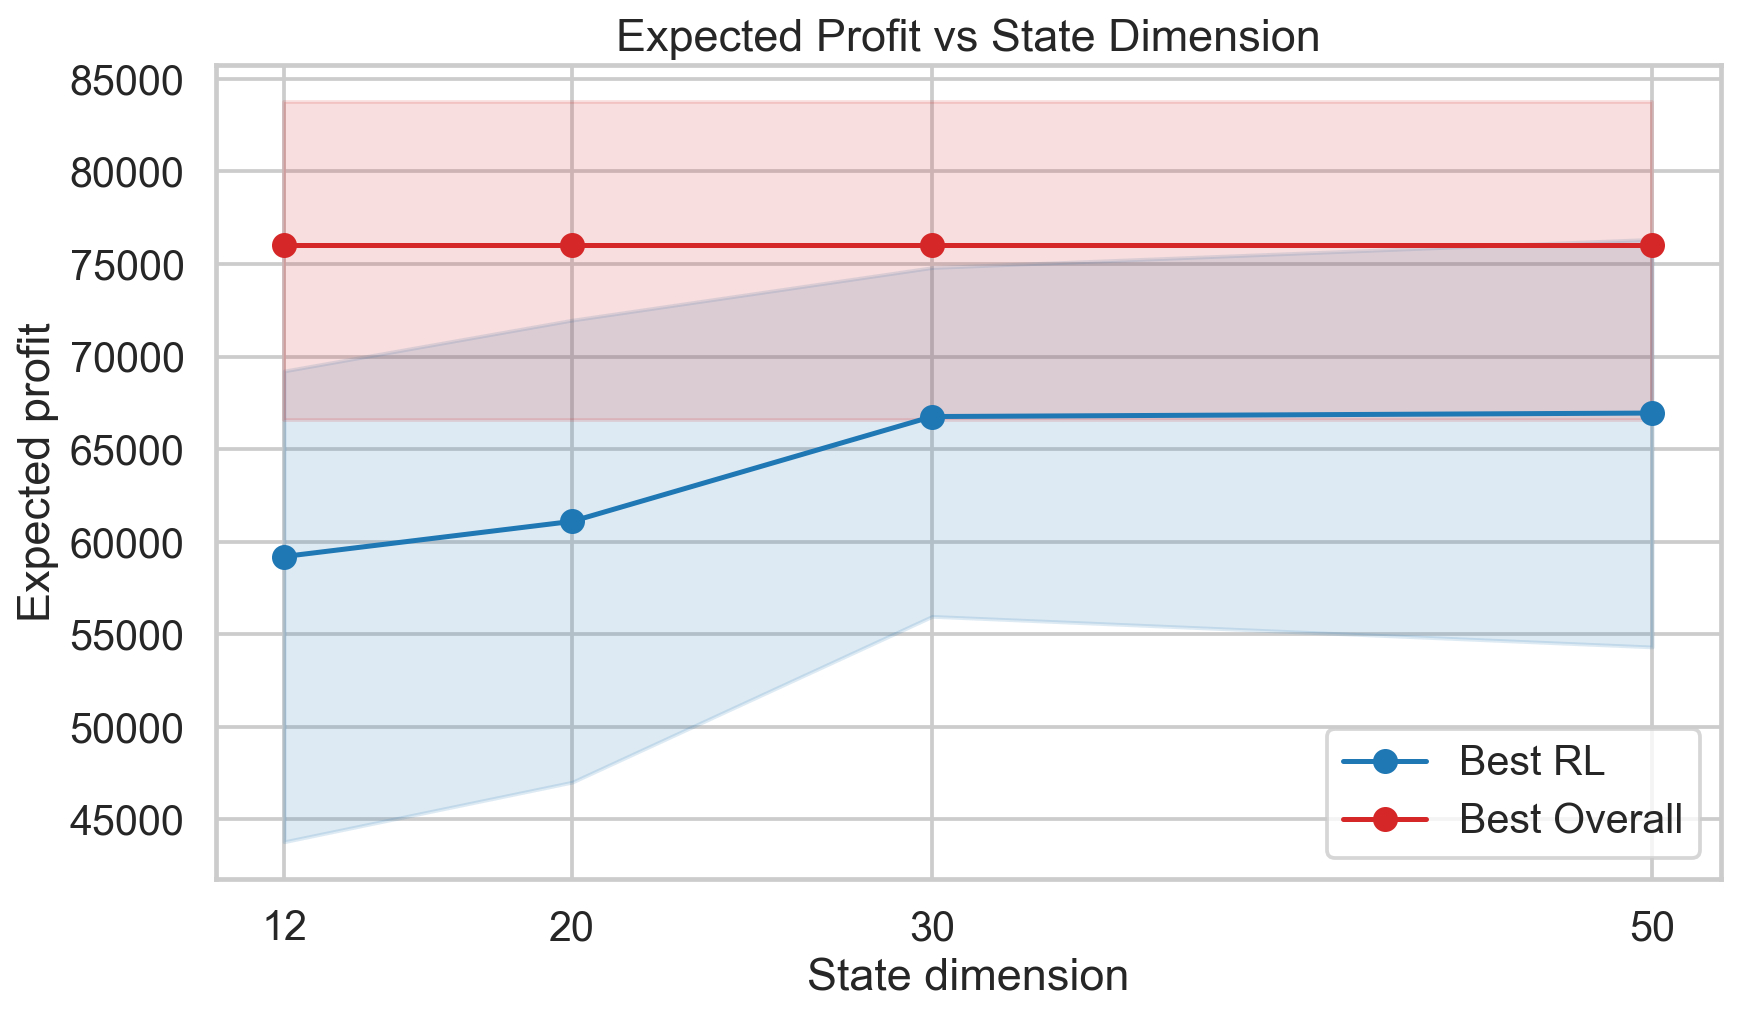
\includegraphics[width=0.82\textwidth]{metric_vs_dimension_expected_profit.png}
    \caption{Прибыль в зависимости от размерности состояния для best RL и best overall controller.}
    \label{fig:ru-profit-vs-dim}
\end{figure}

\begin{figure}[H]
    \centering
    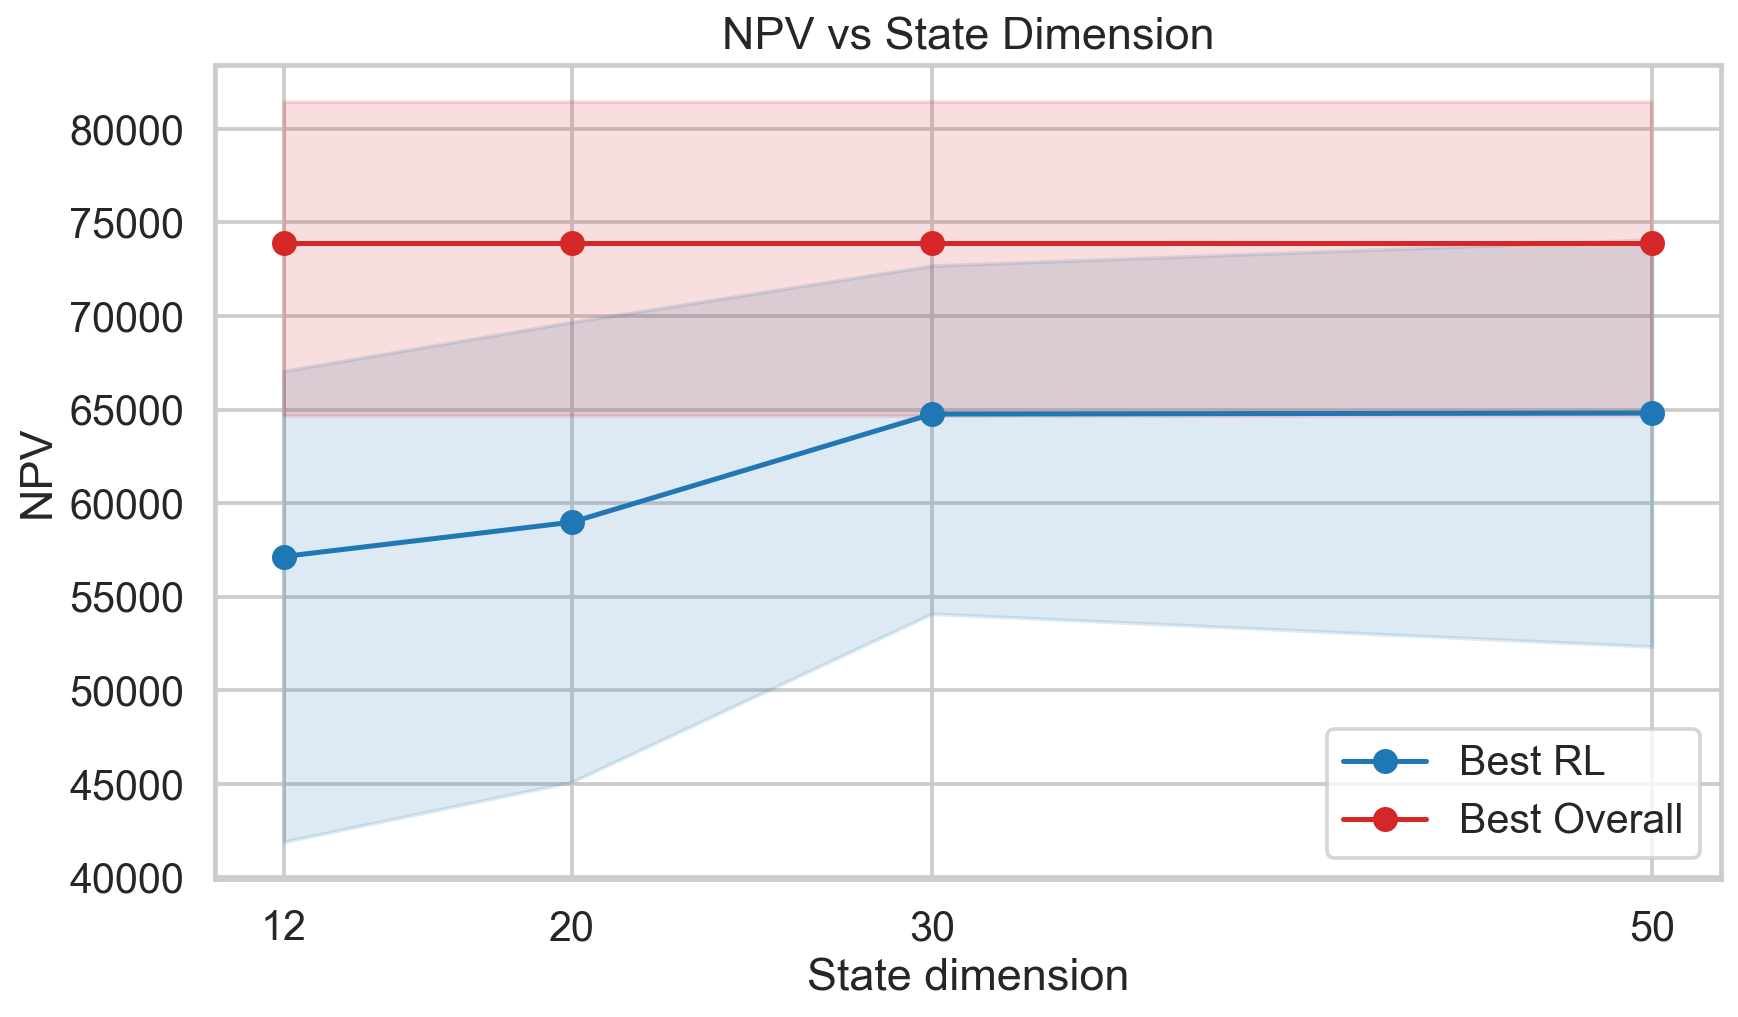
\includegraphics[width=0.82\textwidth]{metric_vs_dimension_npv.png}
    \caption{NPV в зависимости от размерности состояния.}
    \label{fig:ru-npv-vs-dim}
\end{figure}

\begin{figure}[H]
    \centering
    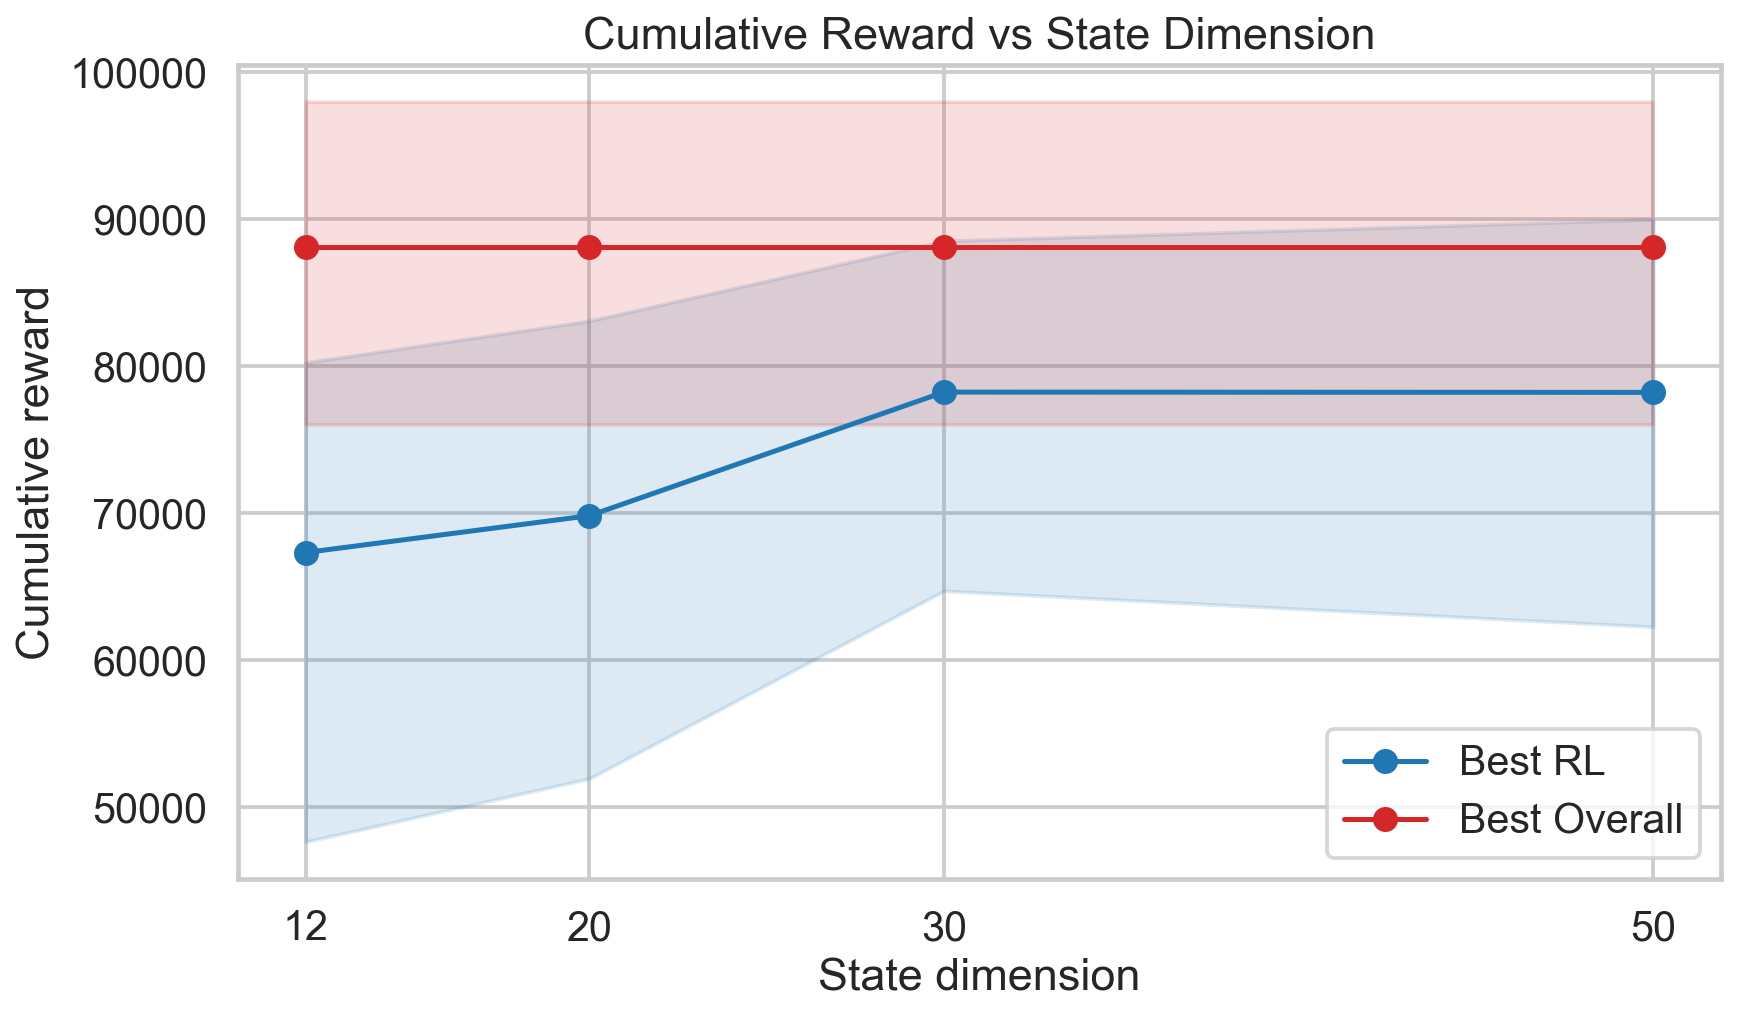
\includegraphics[width=0.82\textwidth]{metric_vs_dimension_cumulative_reward.png}
    \caption{Cumulative reward в зависимости от размерности состояния.}
    \label{fig:ru-reward-vs-dim}
\end{figure}

\begin{figure}[H]
    \centering
    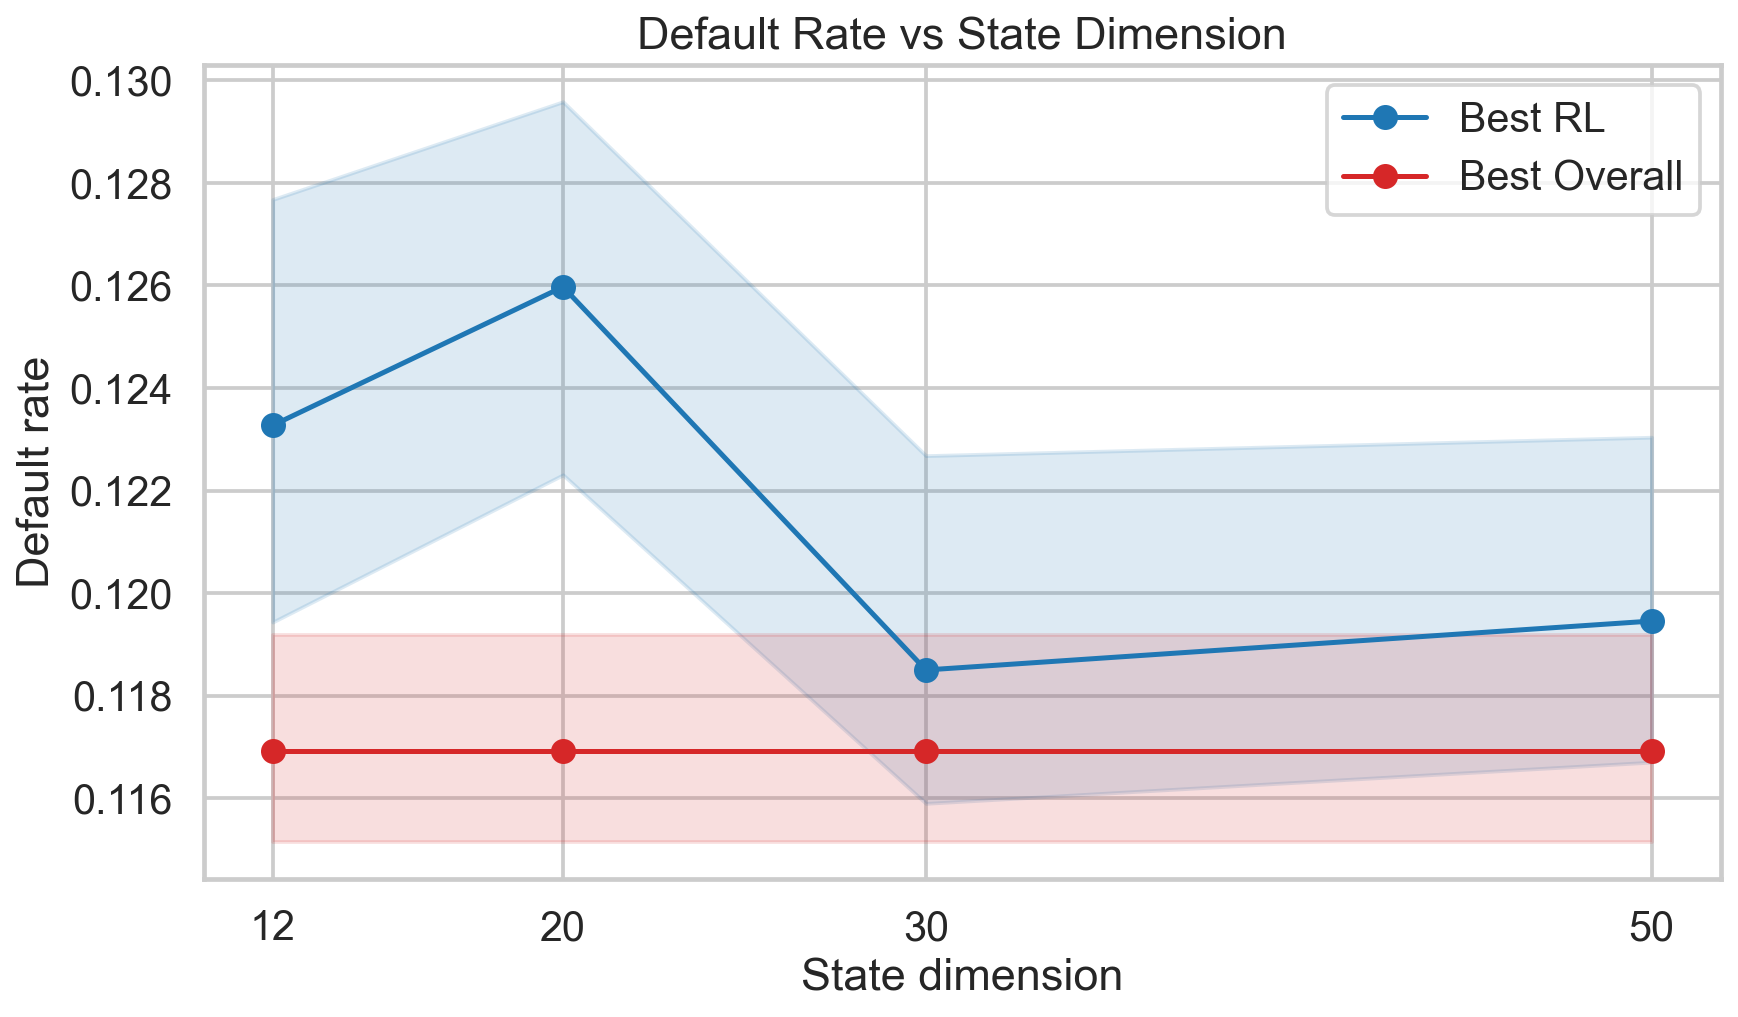
\includegraphics[width=0.82\textwidth]{metric_vs_dimension_default_rate.png}
    \caption{Default rate в зависимости от размерности состояния.}
    \label{fig:ru-default-vs-dim}
\end{figure}

\begin{figure}[H]
    \centering
    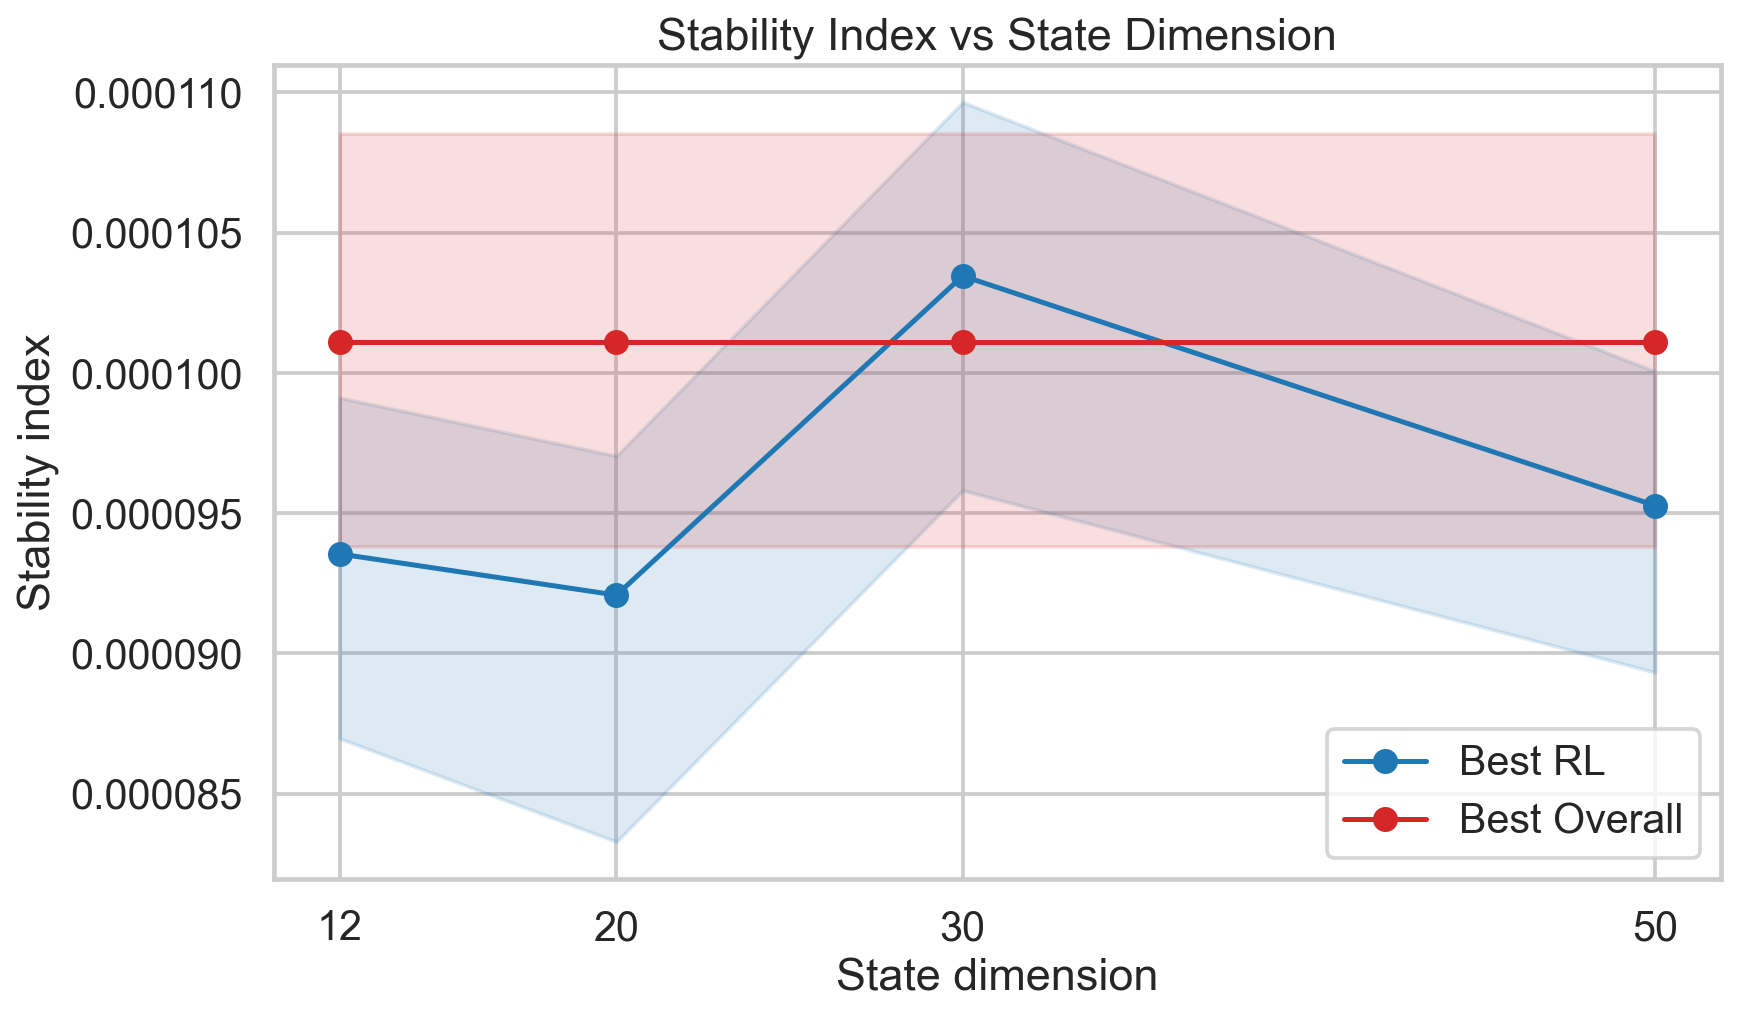
\includegraphics[width=0.82\textwidth]{metric_vs_dimension_stability_index.png}
    \caption{Stability index в зависимости от размерности состояния.}
    \label{fig:ru-stability-vs-dim}
\end{figure}

Эти рисунки вместе очень наглядны. Плоская линия overall-best baseline означает, что comparison set действительно не меняется с ростом размерности. Растущая, а затем выравнивающаяся линия best RL означает, что additional state signal сначала помогает, а затем перестает заметно улучшать управление. Default-rate curve показывает, что ключевой выигрыш достигается к 30D. Stability-index figure показывает, что главное улучшение идет не через радикальный скачок устойчивости, а через лучшую комбинацию profit, selectivity и capital discipline.

\section{Сценарная интерпретация результатов}

\subsection{Почему одной общей таблицы недостаточно}

Overall-ranking полезен, но он скрывает важную структуру. Разные сценарии моделируют разные типы сложности: стабильный режим, медленный drift, сильный shock, composition shift, noise и diverging segment dynamics. Поэтому у исследования неизбежно возникает второй уровень анализа: нужно понять, в каких именно сценариях RL уже близок к baseline, в каких он действительно лучше, а в каких заметно уступает.

Кроме того, необходимо различать по крайней мере три понятия ``лидера'':
\begin{itemize}[leftmargin=*]
    \item reward-based winner;
    \item highest-profit winner;
    \item lowest-default winner.
\end{itemize}

В shaped portfolio problem это не одно и то же.

\subsection{Смысловая карта сценариев в 50D}

\begin{table}[H]
    \centering
    \small
    \begin{tabular}{p{0.21\textwidth}p{0.20\textwidth}p{0.21\textwidth}p{0.20\textwidth}}
        \toprule
        Сценарий & Reward-based winner & Highest-profit winner & Lowest-default winner \\
        \midrule
        \texttt{adverse\_stress} & \texttt{static\_threshold} & \texttt{constraint\_aware\_weekly} & \texttt{risk\_aware\_weekly} \\
        \texttt{base\_market} & \texttt{profit\_oriented} & \texttt{profit\_oriented} & \texttt{risk\_aware\_weekly} \\
        \texttt{class\_imbalance\_shift} & \texttt{constraint\_aware\_weekly} & \texttt{profit\_oriented} & \texttt{risk\_aware\_weekly} \\
        \texttt{drift} & \texttt{profit\_oriented} & \texttt{profit\_oriented} & \texttt{risk\_aware\_weekly} \\
        \texttt{noise} & \texttt{profit\_oriented} & \texttt{profit\_oriented} & \texttt{risk\_aware\_weekly} \\
        \texttt{split\_policy\_dynamics} & \texttt{constraint\_aware\_weekly} & \texttt{profit\_oriented} & \texttt{risk\_aware\_weekly} \\
        \bottomrule
    \end{tabular}
    \caption{Различие между reward, profit и risk лидерами в 50D на основе \texttt{outputs/dim\_50/main\_scenario\_summary.csv}.}
    \label{tab:ru-scenario-50}
\end{table}

Эта таблица очень полезна для объяснения результатов комиссии. Она показывает, что в исследовании нет одного универсального ``победителя''. В стабильном рынке RL действительно может оказаться лучшим и по reward, и по profit, и по default rate одновременно. В noise-сценарии highest-profit winner и reward-based winner расходятся. В class-imbalance-shift conservative baseline выигрывает по profit и reward, а DQN при этом дает наименьший default rate. Именно в таких случаях особенно хорошо виден содержательный trade-off, заложенный в дизайн исследования.

\subsection{Adverse stress}

Во всех размерностях adverse stress остается самой трудной средой для RL. Reward-based winner здесь всегда --- \texttt{profit\_oriented}, с прибылью около $29{,}336.42$, cumulative reward около $25{,}150.74$ и default rate около $0.1178$. Лучшие RL-значения значительно хуже: в 12D best RL имеет отрицательную прибыль, в 30D DQN поднимается лишь до $3{,}413.22$, а в 50D DQN снова уходит в отрицательную прибыль.

Такая картина логична. В adverse stress одновременно растут default pressure, noise и размер кредитной нагрузки. Цена ошибки становится очень высокой. Миопический на вид baseline \texttt{profit\_oriented} здесь на самом деле быстро становится строгим, потому что уже текущая когорта выглядит существенно хуже. Он поджимает выдачу и за счет этого защищает портфель. RL в quick-profile partly учится той же логике, но в условиях короткого training budget не успевает consistently превратить richer state в столь же robust control.

\subsection{Base market}

Base market --- это сценарий, в котором RL выглядит наиболее убедительно. Уже в 12D DQN выигрывает по reward. В 20D strongest RL становится Double-DQN с прибылью $94{,}321.51$. В 50D DQN получает примерно $92{,}105.55$ прибыли, $110{,}521.41$ cumulative reward и default rate $0.1134$, то есть оказывается лучше \texttt{profit\_oriented} одновременно по нескольким ключевым метрикам.

Почему это правдоподобно? Потому что base market дает контроллеру наиболее ``чистый'' режим, где полезный сигнал не заслоняется сильной структурной поломкой. В такой среде richer state действительно может позволить RL найти более тонкую границу селективности, чем rule-based weekly search, и извлечь выгоду из информационной структуры состояния.

\subsection{Class-imbalance shift}

В этом сценарии неизменно побеждает \texttt{constraint\_aware\_weekly}. Это очень содержательный результат. Сценарий специально наказывает политику, которая плохо реагирует на рост доли более слабого сегмента новых клиентов. Явно constraint-aware search здесь естественным образом оказывается очень сильным baseline.

Но одновременно видно, что richer-state DQN приближается к нему и по мере роста размерности сильно улучшает свой результат. В 50D DQN доходит примерно до $65{,}715.59$ по прибыли и одновременно становится lowest-default winner с default rate около $0.1163$. Это означает, что более богатое состояние помогает RL лучше видеть composition risk, хотя quick-profile все еще не дает ему выиграть по главной reward-based ranking.

\subsection{Drift}

Drift особенно важен для интерпретации 30D. Здесь \texttt{profit\_oriented} остается reward-based winner, но best RL profit заметно растет от 12D к 30D и затем ослабевает на 50D. Такая форма полностью соответствует интуиции о значении исторических признаков: медленное ухудшение качества лучше всего ловится тогда, когда в состоянии появляется память о недавней динамике. Именно это и происходит на уровне 30D.

50D в этом сценарии уже не дает сопоставимого прироста. Значит, ключевой полезный signal для drift-среды уже содержится в историческом блоке 30D, а дальнейшее усложнение описания не увеличивает качество управления в той же мере.

\subsection{Noise}

Noise-сценарий особенно полезен для объяснения, что reward и profit --- разные вещи. Highest-profit winner здесь --- \texttt{risk\_aware\_weekly} с прибылью около $97{,}377.95$. Но reward-based winner --- \texttt{profit\_oriented}. Одновременно 30D и 50D DQN показывают очень неплохую прибыль и при этом более низкий default rate, чем у risk-aware baseline.

Это и есть практический смысл исследования: иногда richer-state RL не является лучшим по основной общей ranking, но создает более чистую кредитную политику, уменьшая дефолтность при вполне конкурентной прибыли. Для банковской интерпретации это очень существенный результат.

\subsection{Split-policy dynamics}

Этот сценарий буквально сконструирован для проверки split-policy logic. Reward-based winner остается \texttt{profit\_oriented}, но с ростом размерности лучший RL-контроллер заметно приближается к нему. В 50D DQN получает примерно $119{,}918.57$ прибыли против $120{,}324.99$ у baseline, то есть gap становится очень маленьким. Более того, именно DQN в 50D показывает здесь наименьший default rate, около $0.1093$.

Это сильный содержательный аргумент в пользу richer segmented state. Когда динамика new и repeat сегментов расходится, более богатое состояние действительно помогает RL почти догнать profit-seeking baseline, а по качеству портфеля даже чуть превзойти его.

\section{Что показывают отдельные рисунки по размерностям}

\begin{figure}[H]
    \centering
    \begin{subfigure}[b]{0.48\textwidth}
        \centering
        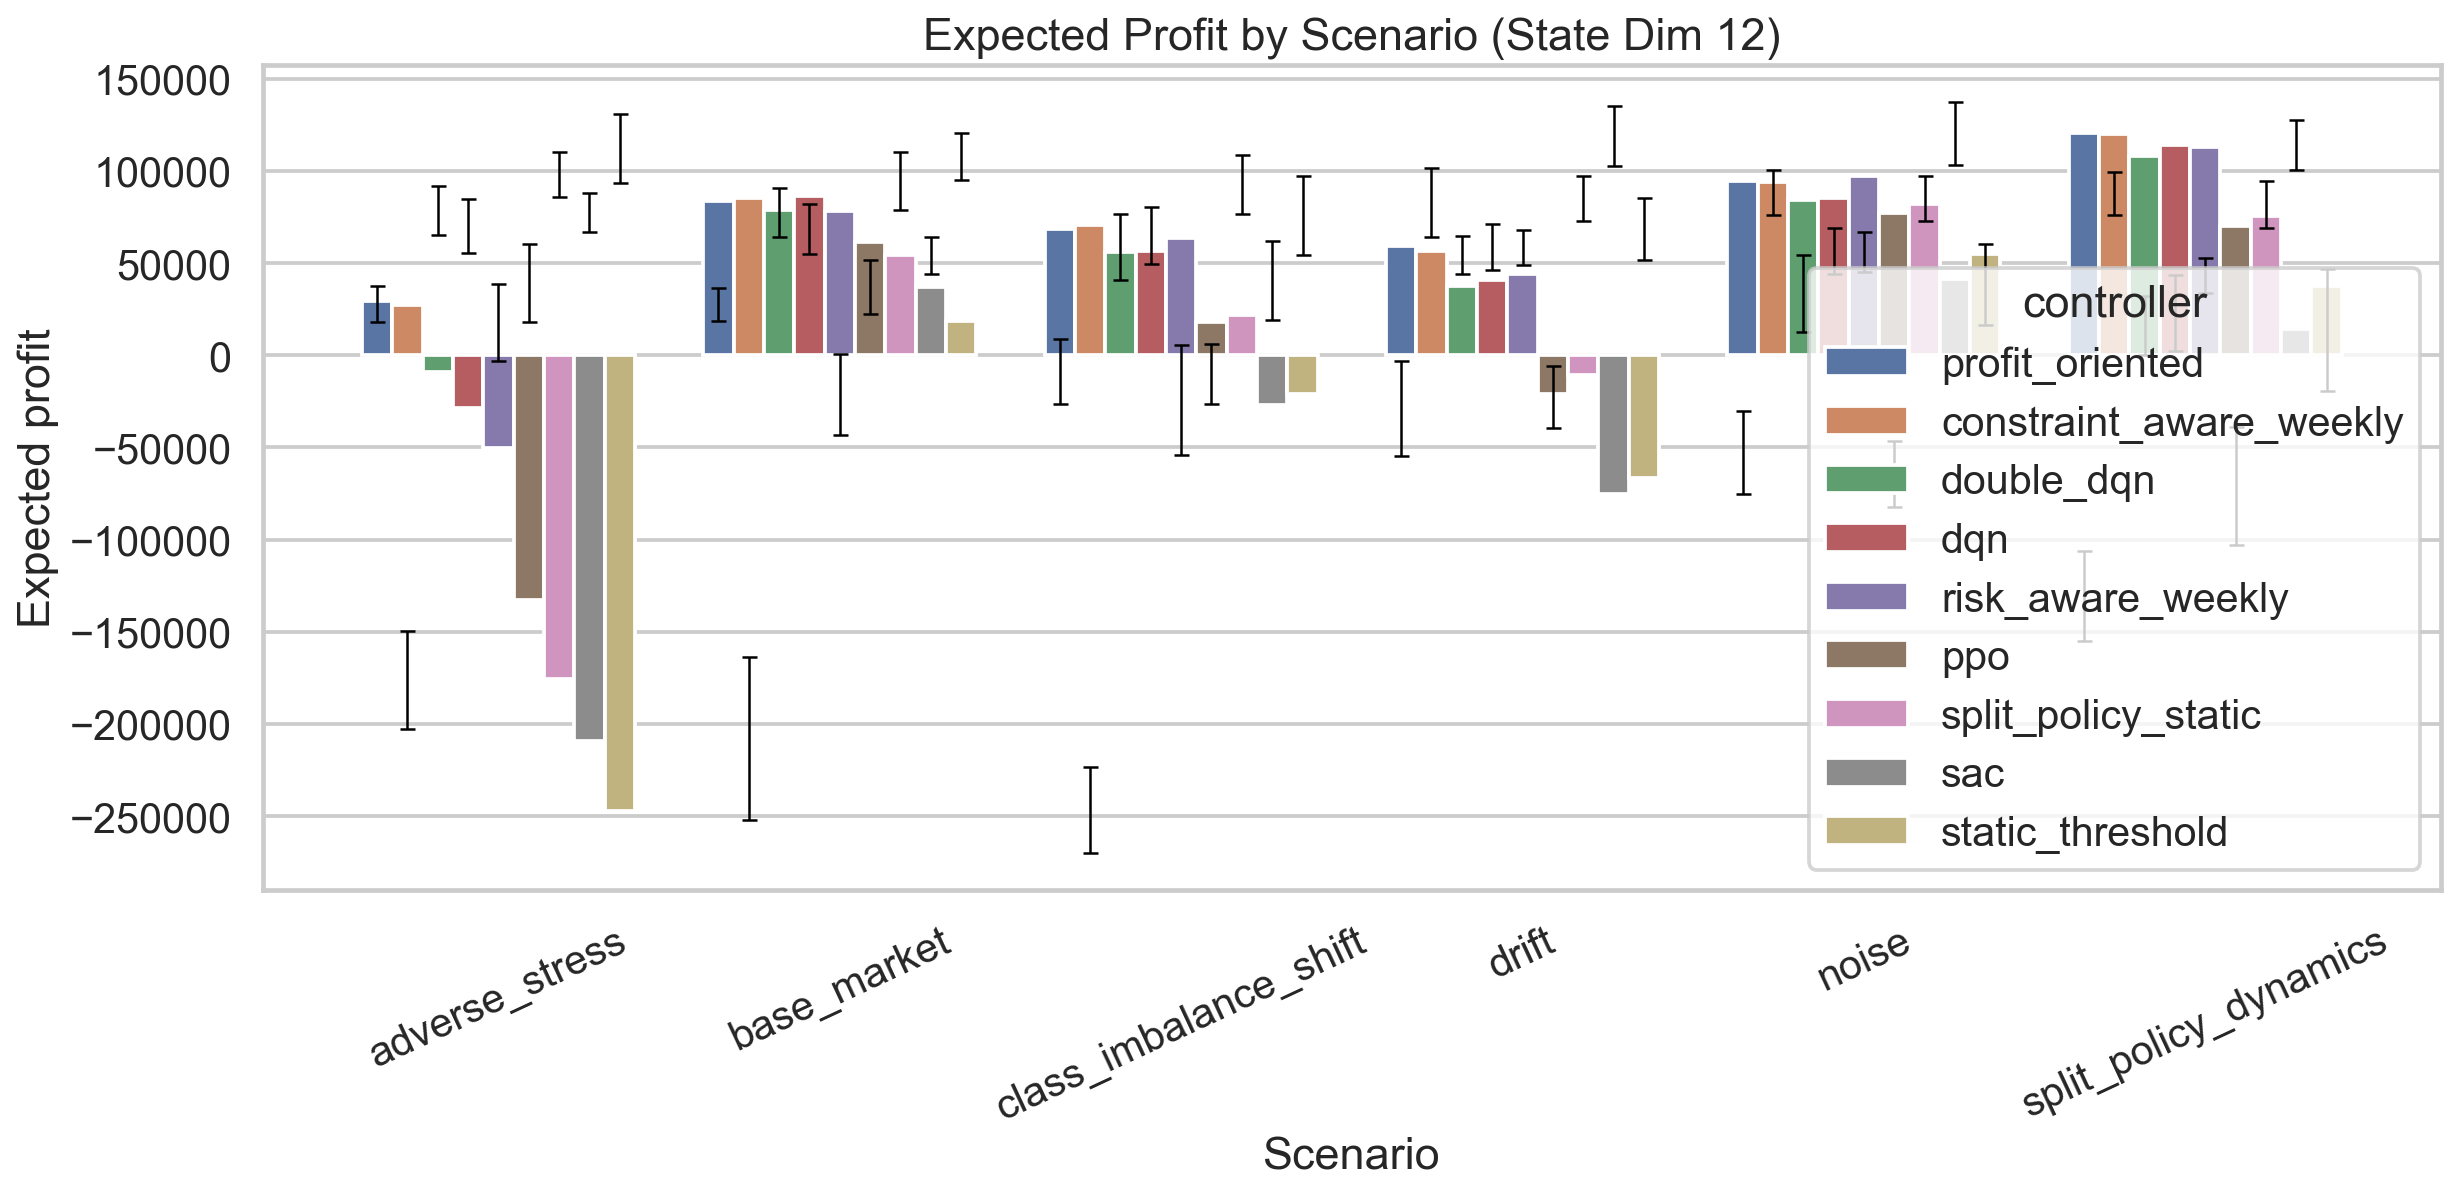
\includegraphics[width=\textwidth]{dim_12/expected_profit_by_scenario_dim12.png}
        \caption{12D}
    \end{subfigure}
    \hfill
    \begin{subfigure}[b]{0.48\textwidth}
        \centering
        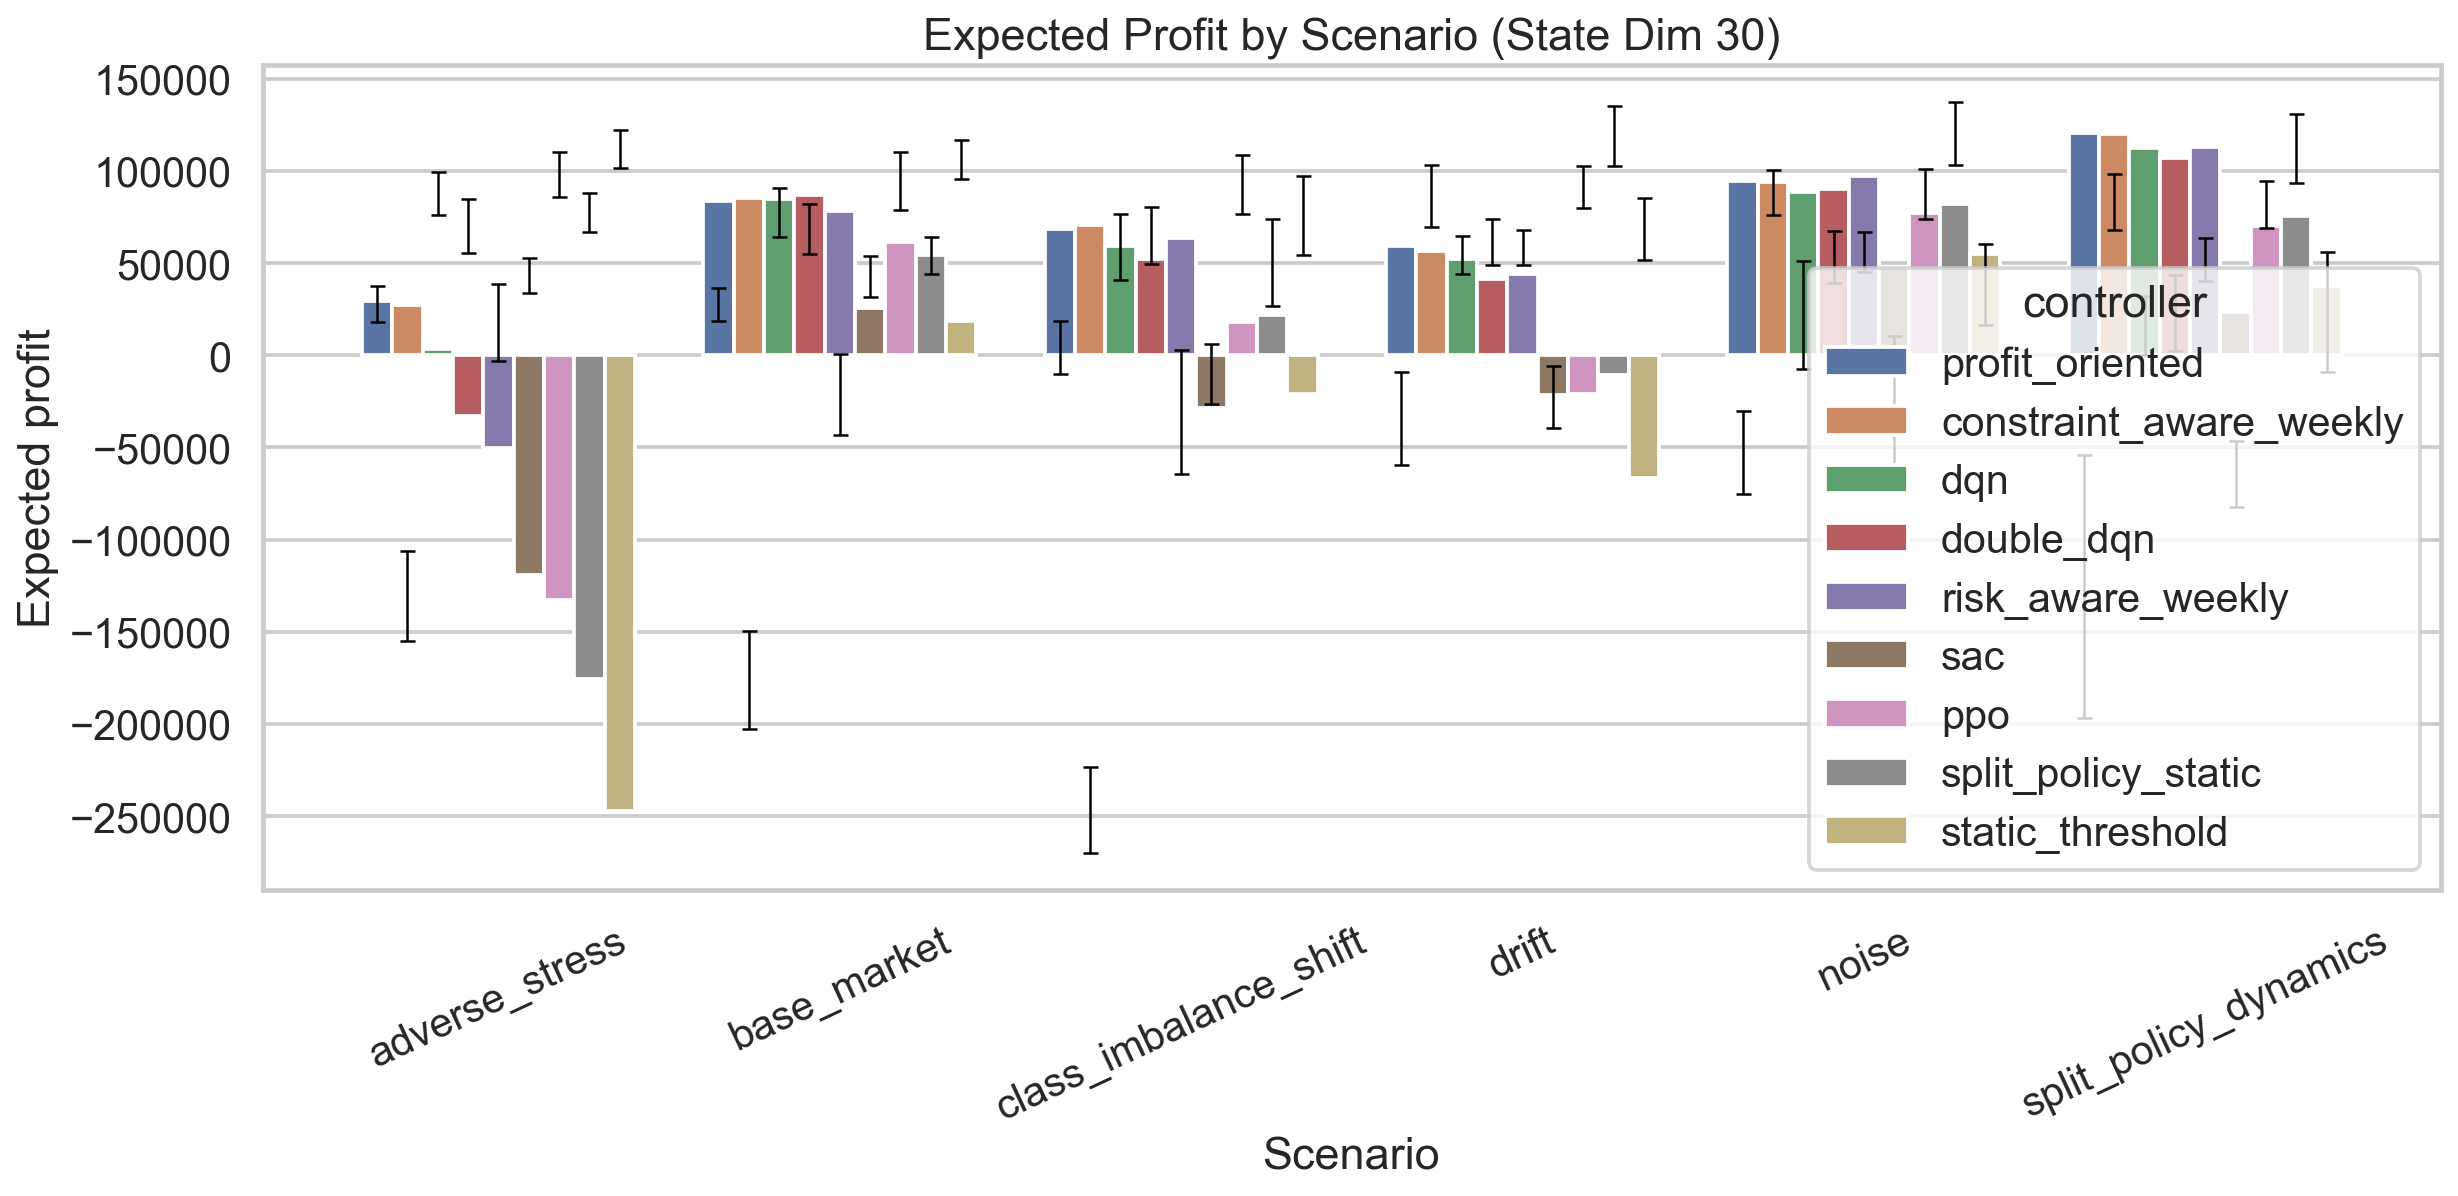
\includegraphics[width=\textwidth]{dim_30/expected_profit_by_scenario_dim30.png}
        \caption{30D}
    \end{subfigure}
    \caption{Scenario-level сравнение прибыли для двух характерных размерностей.}
    \label{fig:ru-profit-scenarios-a}
\end{figure}

\begin{figure}[H]
    \centering
    \begin{subfigure}[b]{0.48\textwidth}
        \centering
        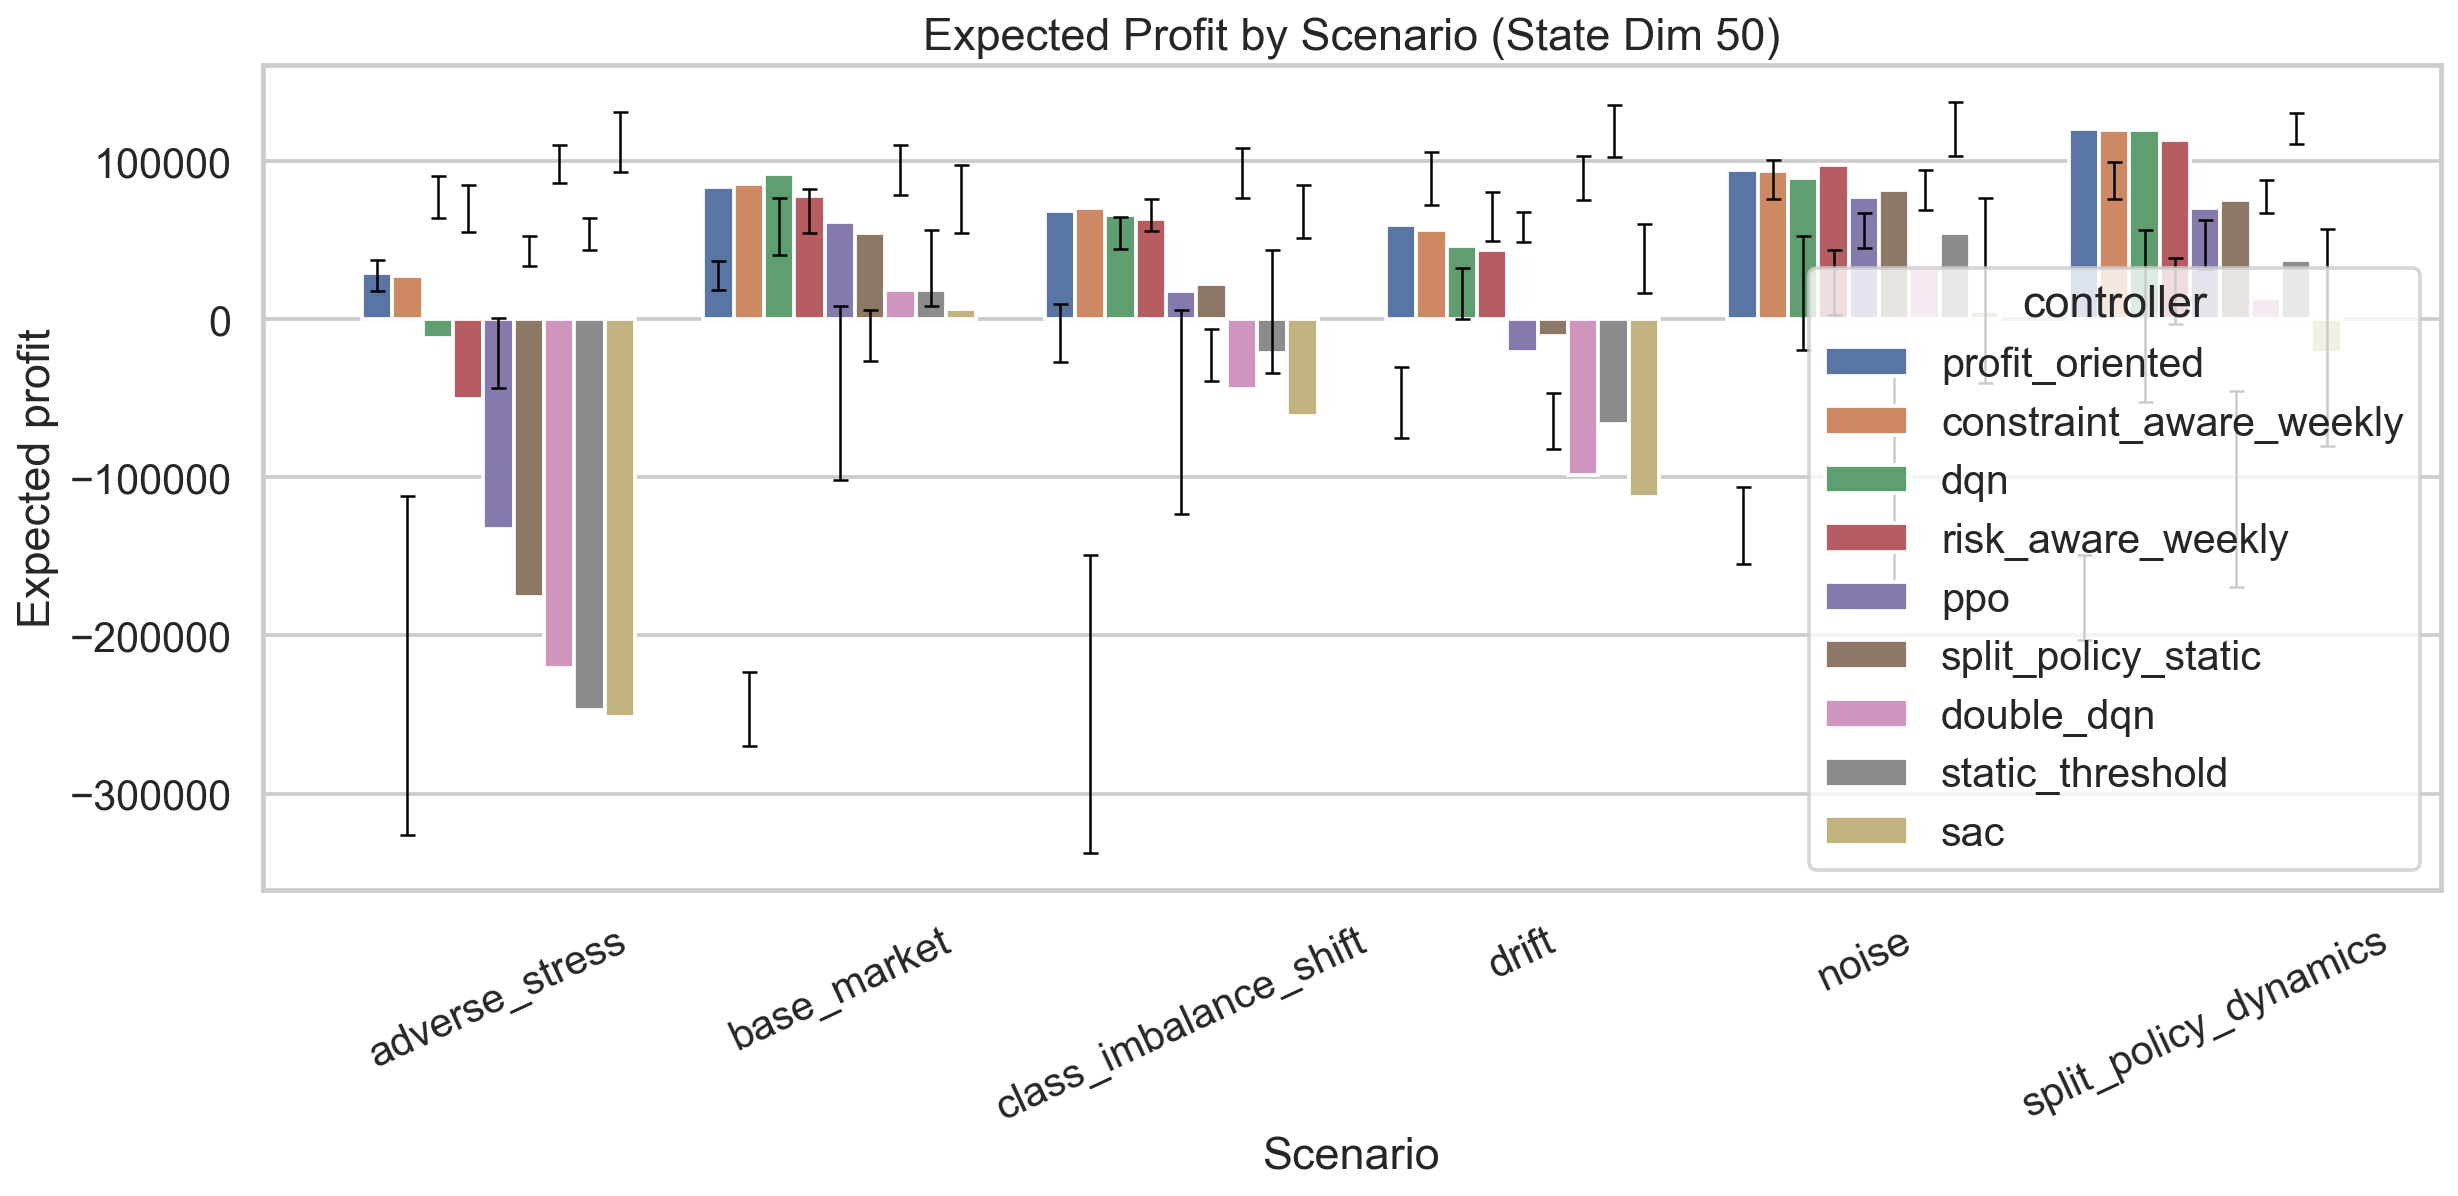
\includegraphics[width=\textwidth]{dim_50/expected_profit_by_scenario_dim50.png}
        \caption{50D profit}
    \end{subfigure}
    \hfill
    \begin{subfigure}[b]{0.48\textwidth}
        \centering
        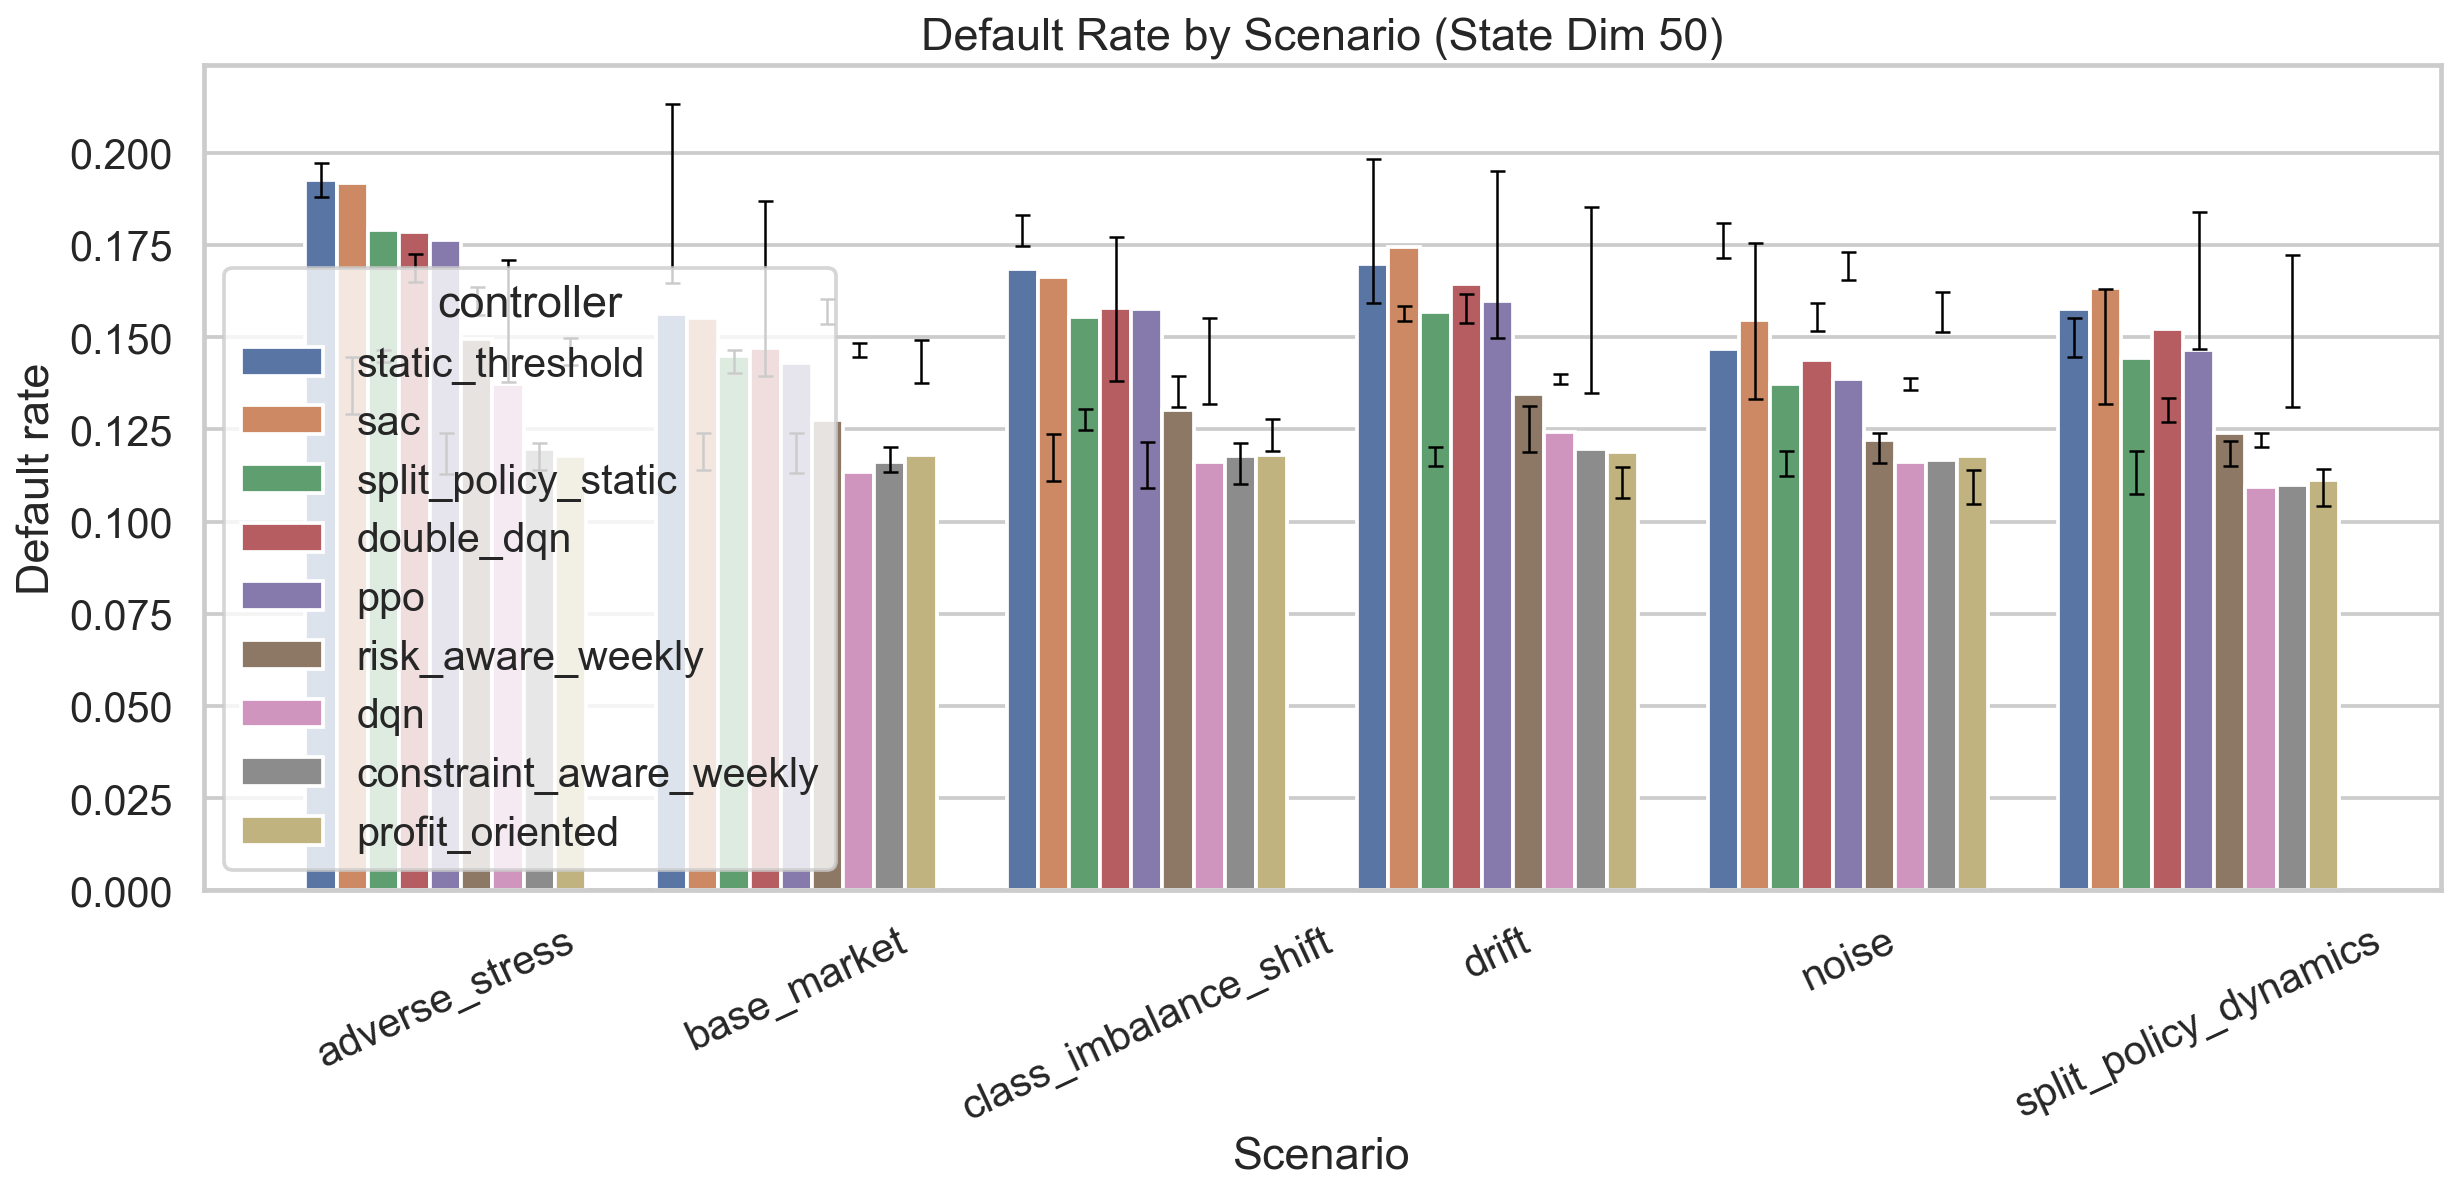
\includegraphics[width=\textwidth]{dim_50/default_rate_by_scenario_dim50.png}
        \caption{50D default rate}
    \end{subfigure}
    \caption{Как богатое состояние меняет баланс между доходностью и риском.}
    \label{fig:ru-profit-scenarios-b}
\end{figure}

\begin{figure}[H]
    \centering
    \begin{subfigure}[b]{0.48\textwidth}
        \centering
        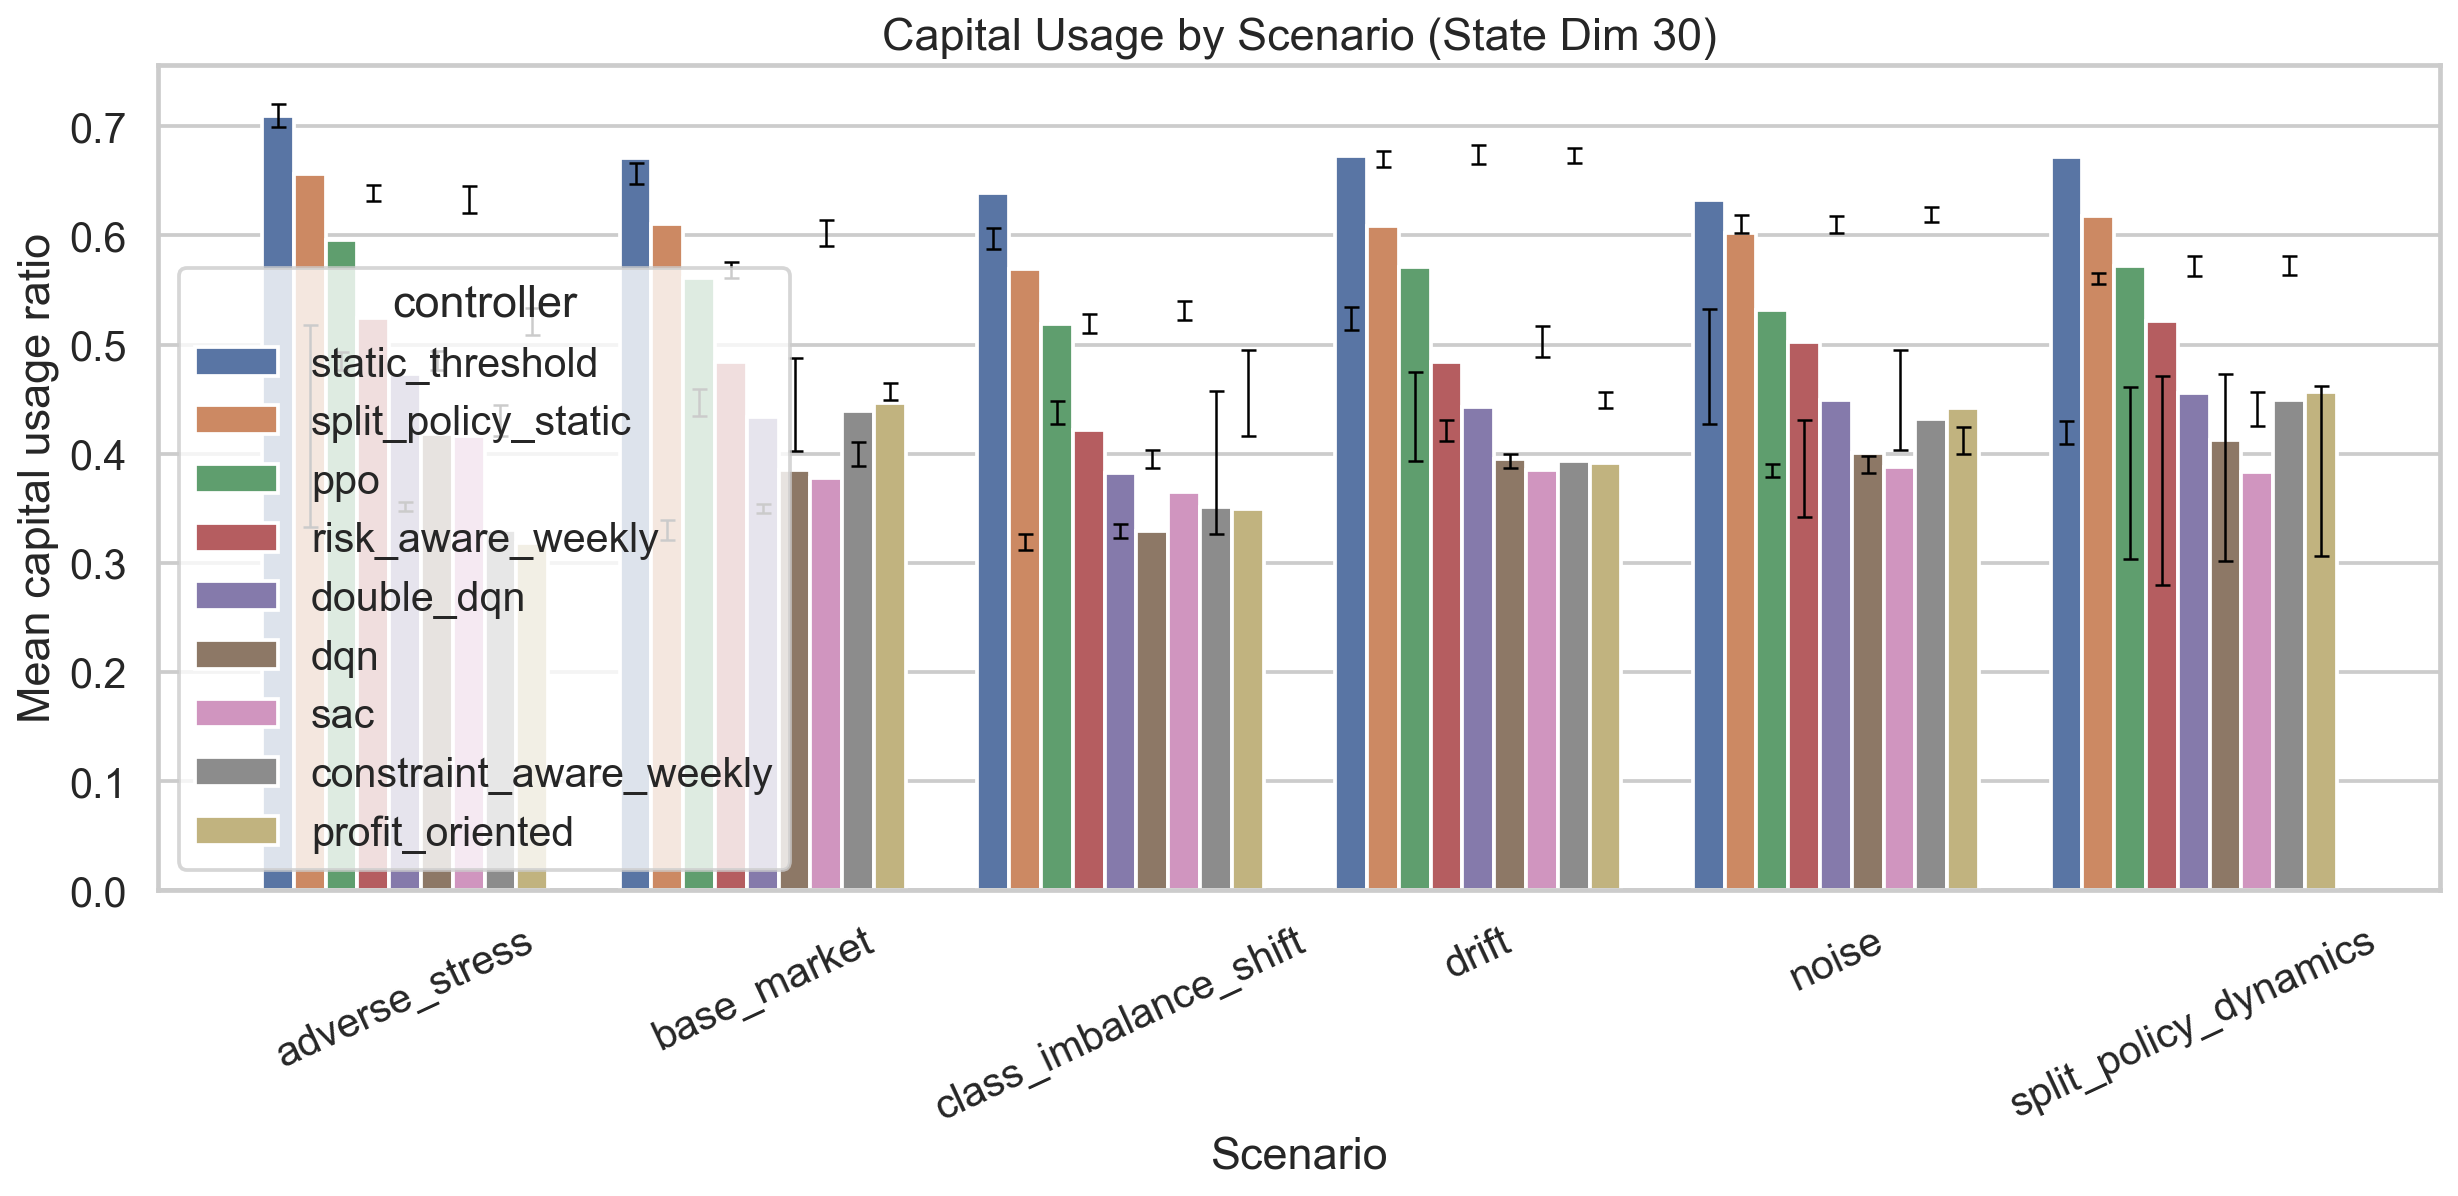
\includegraphics[width=\textwidth]{dim_30/capital_usage_by_scenario_dim30.png}
        \caption{30D capital usage}
    \end{subfigure}
    \hfill
    \begin{subfigure}[b]{0.48\textwidth}
        \centering
        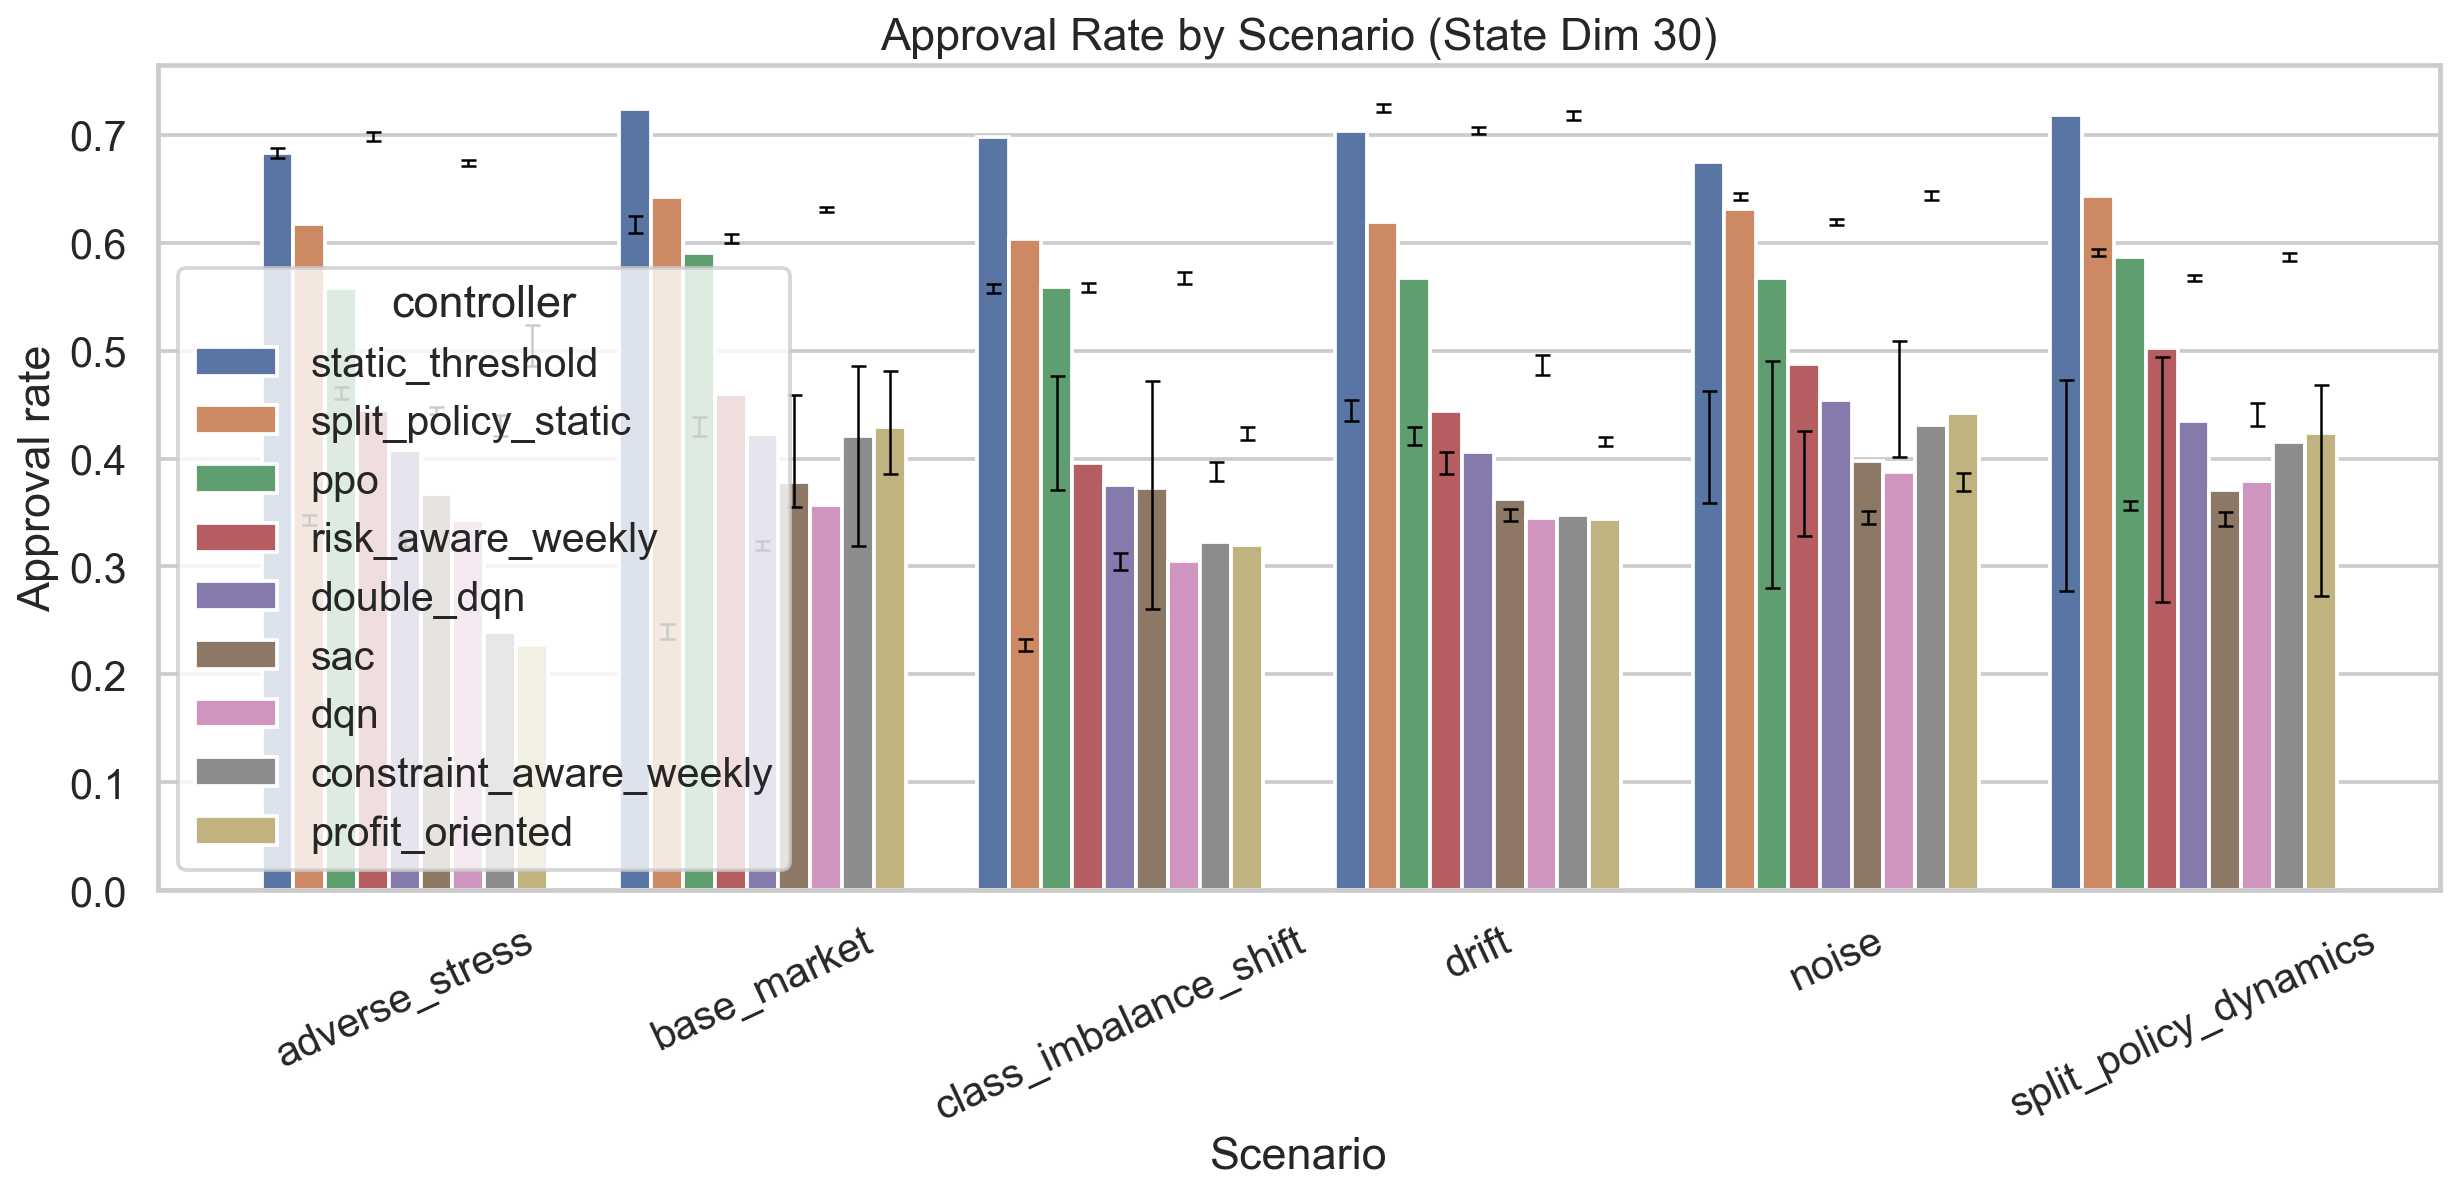
\includegraphics[width=\textwidth]{dim_30/approval_rate_by_scenario_dim30.png}
        \caption{30D approval rate}
    \end{subfigure}
    \caption{Как 30D меняет селективность и загрузку капитала.}
    \label{fig:ru-cap-approval}
\end{figure}

Эти рисунки полезны тем, что позволяют увидеть \emph{структуру} улучшений. Например, 30D не просто ``улучшает среднюю метрику'', а делает RL более селективным и более аккуратным по capital usage. 50D, напротив, показывает, что дальнейший рост сложности уже не приводит к столь же качественному улучшению профиля политики.

\section{Поведение порогов и важная интерпретационная деталь}

\subsection{Почему нулевая threshold volatility не означает полное отсутствие различий}

В aggregated summary у лучших RL-строк \texttt{threshold\_volatility\_mean} равна нулю. Это не означает, что все RL-агенты выбирают один и тот же порог. Это означает, что внутри каждого эпизода порог по неделям не меняется.

Данные weekly logs подтверждают, что для best RL controller в каждой размерности 100\% evaluation episodes являются constant-threshold episodes. Это очень важное наблюдение. В quick-profile richer state улучшает прежде всего \emph{выбор удачной пары порогов на эпизод}, а не обучение по-настоящему ``живой'' weekly-adaptive траектории.

\subsection{Какие пороговые пары выбирают лучшие RL-контроллеры}

Экспорт weekly logs показывает следующие типичные пары.
\begin{itemize}[leftmargin=*]
    \item 12D DQN: $(65,45)$, $(85,35)$, $(85,50)$.
    \item 20D Double-DQN: $(65,40)$, $(75,50)$, $(80,55)$.
    \item 30D DQN: $(70,65)$, $(85,35)$, $(85,50)$.
    \item 50D DQN: $(70,45)$, $(85,40)$, $(85,45)$.
\end{itemize}

Это observation полезно для очень честной академической интерпретации. Текущие результаты сильнее подтверждают тезис ``лучшее состояние помогает выбрать лучшую split-policy конфигурацию'', чем тезис ``лучшее состояние уже приводит к сложной адаптивной weekly-control траектории''. Для quick-profile это важная граница корректного вывода.

\subsection{Почему это все равно важный результат}

Даже если best RL policy внутри эпизода почти не двигает thresholds, это не обесценивает исследование. Напротив, это показывает, что при текущем training budget основной выигрыш приходит от более качественного \emph{policy selection}, а не от интенсивной week-to-week корректировки. Для диплома это полезно: можно честно показать и сильную сторону RL-state design, и текущую эмпирическую границу его адаптивности.

\section{Обсуждение}

\subsection{Почему 30D выглядит наиболее сбалансированной размерностью}

30D --- это точка, в которой richer state еще добавляет значимый полезный signal, но еще не создает чрезмерной optimization complexity. Именно здесь наблюдается самый сильный скачок по лучшему RL reward, существенный рост прибыли и NPV, снижение default rate относительно 20D и одновременное сокращение approval rate и capital usage. Такой набор движений особенно важен: он показывает, что контроллер не ``покупает'' reward за счет более агрессивной выдачи, а улучшает качество отбора.

Содержательно это очень хорошо согласуется с природой added features. Между 20D и 30D в состояние добавляется историческая память: лаги по approval/default/profit/capital usage, rolling means, rolling std по прибыли и lagged threshold deltas. Для недельной портфельной задачи это, вероятно, наиболее ценный дополнительный блок.

\subsection{Почему 50D выглядит как saturation, а не как новый скачок}

50D добавляет сегментную детализацию, rolling reward features, cumulative-to-date metrics и историю threshold-gap. Эти признаки не бессмысленны. Но в текущем quick-profile они почти не двигают best RL frontier дальше. Более того, для части алгоритмов 50D оказывается даже вредным.

Это особенно видно по Double-DQN: он лучший RL на 20D, терпимый на 30D и катастрофически плохой на 50D. Следовательно, рост размерности здесь нужно понимать не как бесплатное обогащение информации, а как совместный рост и signal, и optimization burden.

\subsection{Почему baseline по-прежнему выигрывает overall}

Лидерство \texttt{profit\_oriented} и близость \texttt{constraint\_aware\_weekly} вполне объяснимы. Эти политики напрямую используют структурную форму задачи.
\begin{itemize}[leftmargin=*]
    \item Они выполняют явный weekly search по той же сетке порогов, которую допускает среда.
    \item Им не нужно учить value function или policy approximation при коротком бюджете.
    \item Их логика напрямую связана с текущей экономикой когорты и с constraint-структурой reward.
\end{itemize}

Поэтому корректный вывод состоит не в том, что RL ``проиграл'', а в том, что в хорошо структурированном simulator strong rule-based policy search остается очень сильным benchmark. RL при этом становится существенно лучше, когда state design становится более информативным.

\subsection{Практический смысл trade-offs}

С прикладной точки зрения один из самых интересных моментов исследования --- это то, как меняются approval rate, capital usage и default rate вместе с ростом размерности. 20D best RL policy становится более одобряющей и более капиталоемкой. 30D best RL policy, наоборот, становится более селективной и одновременно более сильной по reward. 50D снова ослабляет эту дисциплину.

Для портфельного кредитного бизнеса это важнее, чем простое сравнение одной метрики. Смысл управления порогом заключается именно в том, чтобы найти workable compromise между объемом выдач, качеством портфеля, устойчивостью и использованием капитала.

\section{Ограничения исследования}

\begin{itemize}[leftmargin=*]
    \item Симулятор синтетический. Он экономически правдоподобен, но не является прямой калибровкой на production-данные банка.
    \item Quick-profile intentionally short. 12 training episodes на seed достаточно для controlled comparison, но недостаточно для сильных заявлений о полном convergence RL.
    \item Функция награды является спроектированной. Следовательно, ranking контроллеров зависит от выбранного баланса между доходностью и штрафами.
    \item Экспортированные CI отражают неопределенность внутри выбранного генератора сценариев, а не внешнюю валидность на реальном рынке.
    \item Лучшие RL-политики в текущем профиле в основном episode-static, поэтому evidence for truly dynamic weekly threshold adjustment пока слабее, чем evidence for better threshold-pair selection.
\end{itemize}

Эти ограничения не разрушают выводы, но задают корректную границу того, что именно уже показано, а что еще требует дальнейшей проверки.

\section{Научная новизна и вклад}

Новизна работы не в придумывании еще одного RL-алгоритма как такового, а в комбинации нескольких исследовательских идей в одной согласованной постановке.
\begin{itemize}[leftmargin=*]
    \item Кредитное управление формулируется как недельное портфельное threshold control, а не как однократная классификация.
    \item Delayed outcomes и terminal settlement встроены в саму среду, а не вынесены в постобработку.
    \item Новые и повторные клиенты моделируются раздельно и управляются через split-policy action.
    \item RL сравнивается не с примитивным baseline, а с набором экономически осмысленных rule-based контроллеров.
    \item Сам state design превращается в самостоятельный объект controlled empirical study.
\end{itemize}

Именно так и следует формулировать contribution диплома: это вклад в problem formulation, simulation design и controlled experimental methodology для RL-based credit policy research.

\section{Заключение}

Текущее состояние репозитория позволяет сделать четкий и хорошо аргументированный вывод. Увеличение размерности состояния с 12 до 20 и затем до 30 признаков существенно улучшает лучшую RL-политику. Наиболее сильный прирост достигается на 30D: растут прибыль, NPV и cumulative reward, одновременно улучшается default profile и снижается capital usage по сравнению с 20D winner. Переход 30D $\rightarrow$ 50D дает уже очень мало дополнительной пользы и показывает явный saturation effect.

При этом исследование не поддерживает упрощенный тезис ``RL уже всегда лучше baseline''. Лучший overall-контроллер в quick-profile outputs --- это по-прежнему \texttt{profit\_oriented} baseline, а \texttt{constraint\_aware\_weekly} находится почти на том же уровне. Зато исследование очень убедительно показывает другое: если задача формулируется как weekly portfolio control с delayed outcomes, то качество RL сильно зависит от того, насколько содержательно сконструировано состояние.

Самый корректный финальный вывод звучит так. В рассматриваемом RL credit-scoring simulator richer state действительно создает полезный сигнал, но только до определенной точки. Исторический и портфельный контекст, добавленный к 30D, дает наибольший прирост качества. Дальнейшее расширение до 50D уже почти не улучшает лучший RL frontier и может ухудшать результат у отдельных алгоритмов. Следовательно, в текущей реализации именно дизайн состояния, а не только выбор алгоритма, является одним из ключевых факторов качества портфельного порогового управления.

\section*{Доступность кода}

Полный исходный код симулятора, конфигурации экспериментов, реализации агентов, пайплайн оценки и выходные артефакты, полученные в рамках данной работы, находятся в открытом доступе по адресу:

\begin{center}
    \href{https://github.com/EvgenyBaulin/Evaluation-of-RL-framework-in-a-credit-scoring-problem}{%
    \texttt{https://github.com/EvgenyBaulin/Evaluation-of-RL-framework-in-a-credit-scoring-problem}}
\end{center}

\bibliographystyle{plain}
\bibliography{references}

\end{document}
